\documentclass[final,3p,times]{elsarticle}
\usepackage[utf8]{inputenc}
\usepackage{amssymb}
\usepackage{float}
\usepackage{placeins}
\usepackage{amsmath}
\usepackage{booktabs}
\usepackage{array}
\usepackage{textcomp}
\usepackage{multirow}
\usepackage{threeparttable}
\usepackage{siunitx}
\usepackage[table]{xcolor}
\usepackage{xurl}
\usepackage{hyperref}
\usepackage{caption}
\pdfstringdefDisableCommands{%
  \def\corref#1{}%
  \def\cnotenum#1{}%
  \def\tnoteref#1{}%
}
%todo*: he.huang 29 August, 3:59 amThe three stratgies are proposed by you right? In the text you should make it explicit the statement from you and evidence from literature.he.huang29 August, 4:00 amAnd I think it is not necessary to bring \mathcal{A}s to the introduction.If you would like to mention the specific criteria and energy related paramters. You should explicitly introduce it [ as in this MAVT framework of the paper] as a energy evaluation framework/model instead of a general MAVT reference frameworkhe.huang29 August, 4:20 amAnother thing is you introudce three arthitecure, if the RQ is to find the best one, then here should be rather an experiement design since at the end you don't really need three arthictectures. Think about it and maybe redesign the flow
%todo*:As said, you shouldn't have subsection right after a section title without any text

\usepackage{pgfplots}
\usepgfplotslibrary{colormaps,groupplots,statistics}
\pgfplotsset{compat=1.18}
\usepackage{tikz}
\usetikzlibrary{shapes,arrows.meta,positioning,fit,backgrounds,calc}
\setlength{\marginparwidth}{2cm}
\usepackage{todonotes}
\usepackage{alltt}
\graphicspath{{./}{Images/}}
\setlength{\textfloatsep}{10pt plus 2pt minus 4pt}   % Distance between top/bottom float and text
\setlength{\floatsep}{8pt plus 2pt minus 2pt}       % Distance between two floats
\setlength{\intextsep}{10pt plus 2pt minus 2pt}     % Distance between inline float and text
\renewcommand{\floatpagefraction}{0.7}
\renewcommand{\textfraction}{0.15}
\renewcommand{\topfraction}{0.85}
\renewcommand{\bottomfraction}{0.65}

\newcommand{\plotCriterionMAEByModel}{%
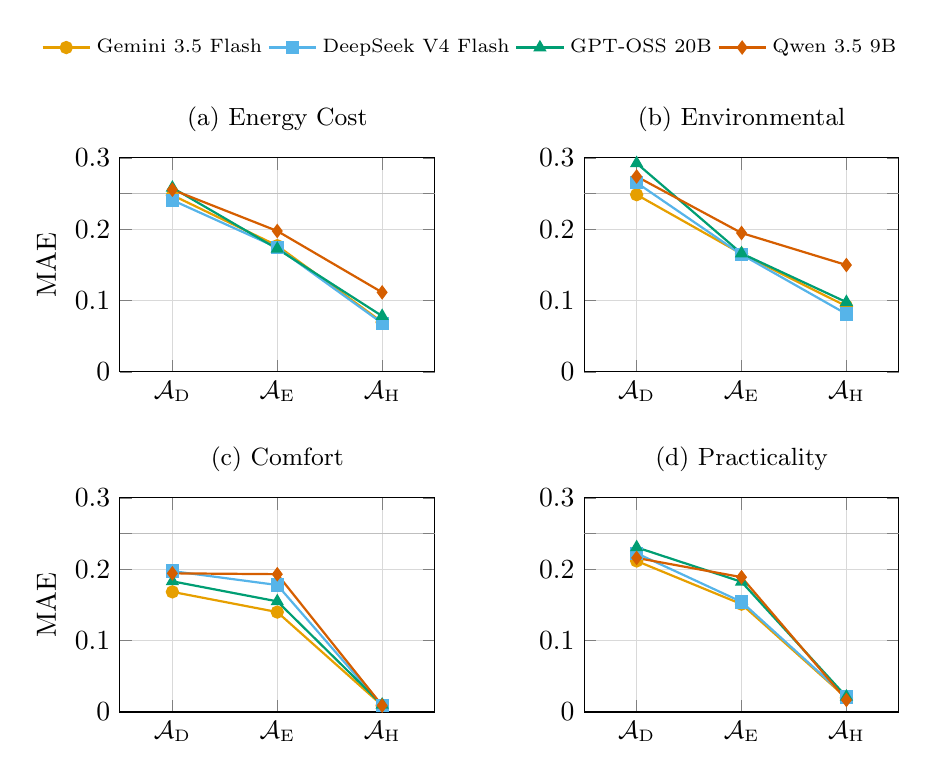
\begin{tikzpicture}
\begin{groupplot}[
    group style={group size=2 by 2, horizontal sep=1.9cm, vertical sep=1.6cm},
    width=0.46\textwidth, height=4.3cm,
    xtick={1,2,3}, xticklabels={$\mathcal{A}_{\text{D}}$,$\mathcal{A}_{\text{E}}$,$\mathcal{A}_{\text{H}}$},
    xticklabel style={font=\small},
    enlarge x limits=0.25,
    grid=major, grid style={gray!30}, ymajorgrids=true,
    extra y ticks={0.25,0.5,0.75},
    extra y tick style={grid=major, grid style={gray!50}},
    extra y tick labels={},
    legend style={font=\scriptsize, at={(1.118,1.42)}, anchor=south, legend columns=4, draw=none, fill=none},
    legend cell align={left},
    every axis plot/.append style={thick, mark size=2pt},
]
\nextgroupplot[ylabel={MAE}, ymin=0, ymax=0.3,
    title={\small (a) Energy Cost}, title style={font=\small}]
\addplot[mark=*, colorGemini]   coordinates {(1,0.2477) (2,0.1769) (3,0.0698)};
\addplot[mark=square*, colorDeepSeek] coordinates {(1,0.2407) (2,0.1742) (3,0.0683)};
\addplot[mark=triangle*, colorGPTOSS] coordinates {(1,0.2581) (2,0.1725) (3,0.0783)};
\addplot[mark=diamond*, colorQwen] coordinates {(1,0.2554) (2,0.1975) (3,0.1115)};
\legend{Gemini 3.5 Flash, DeepSeek V4 Flash, GPT-OSS 20B, Qwen 3.5 9B}
\nextgroupplot[ylabel={}, ymin=0, ymax=0.3,
    title={\small (b) Environmental}, title style={font=\small}]
\addplot[mark=*, colorGemini]   coordinates {(1,0.2484) (2,0.1655) (3,0.0921)};
\addplot[mark=square*, colorDeepSeek] coordinates {(1,0.2652) (2,0.1645) (3,0.0812)};
\addplot[mark=triangle*, colorGPTOSS] coordinates {(1,0.2924) (2,0.1661) (3,0.0978)};
\addplot[mark=diamond*, colorQwen] coordinates {(1,0.2739) (2,0.1947) (3,0.1498)};
\nextgroupplot[ylabel={MAE}, ymin=0, ymax=0.3,
    title={\small (c) Comfort}, title style={font=\small}]
\addplot[mark=*, colorGemini]   coordinates {(1,0.1683) (2,0.1400) (3,0.0091)};
\addplot[mark=square*, colorDeepSeek] coordinates {(1,0.1974) (2,0.1779) (3,0.0089)};
\addplot[mark=triangle*, colorGPTOSS] coordinates {(1,0.1831) (2,0.1550) (3,0.0101)};
\addplot[mark=diamond*, colorQwen] coordinates {(1,0.1943) (2,0.1931) (3,0.009)};
\nextgroupplot[ylabel={}, ymin=0, ymax=0.3,
    title={\small (d) Practicality}, title style={font=\small}]
\addplot[mark=*, colorGemini]   coordinates {(1,0.2116) (2,0.1511) (3,0.0197)};
\addplot[mark=square*, colorDeepSeek] coordinates {(1,0.2224) (2,0.1543) (3,0.0208)};
\addplot[mark=triangle*, colorGPTOSS] coordinates {(1,0.2307) (2,0.1824) (3,0.0213)};
\addplot[mark=diamond*, colorQwen] coordinates {(1,0.2159) (2,0.1889) (3,0.0168)};
\end{groupplot}
\end{tikzpicture}%
}

\newcommand{\plotDecisionTypeByModel}{%
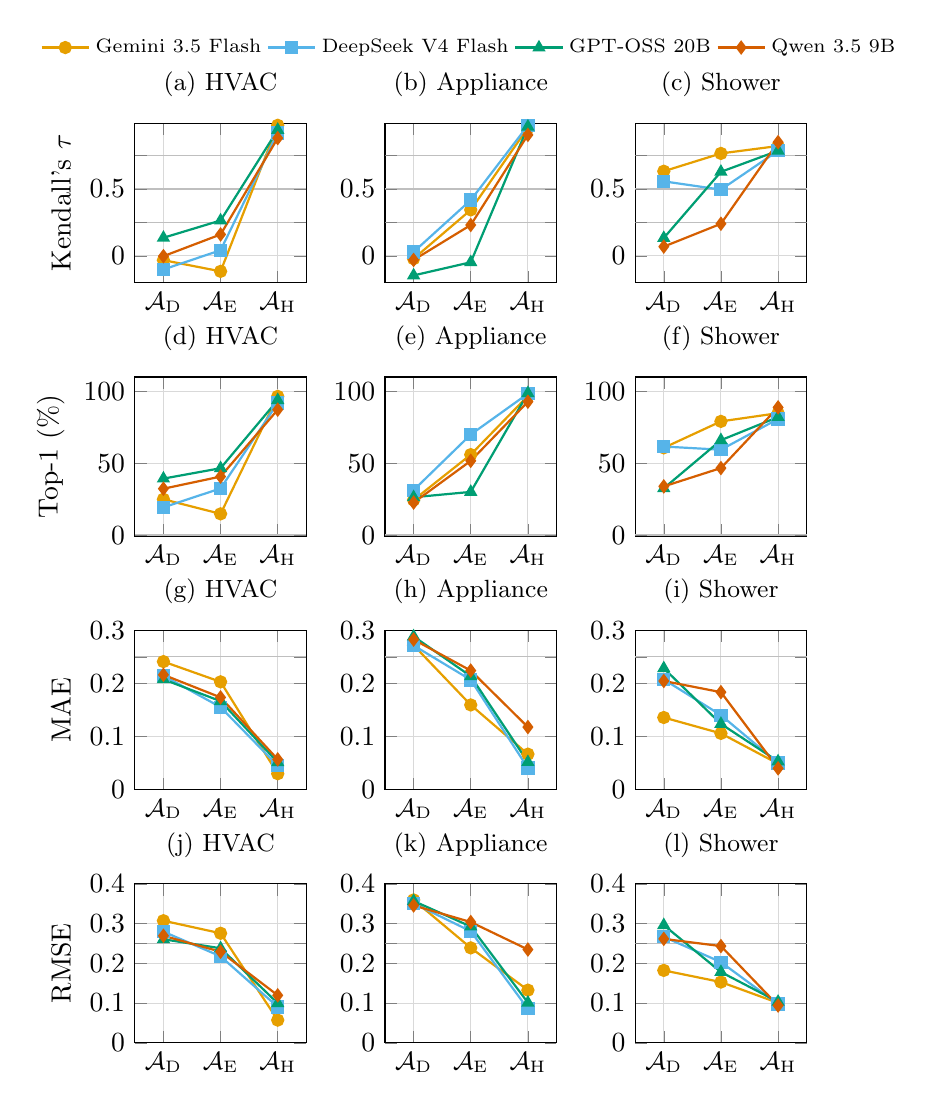
\begin{tikzpicture}
\begin{groupplot}[
    group style={group size=3 by 4, vertical sep=1.2cm},
    width=0.31\textwidth, height=3.6cm,
    xtick={1,2,3}, xticklabels={$\mathcal{A}_{\text{D}}$,$\mathcal{A}_{\text{E}}$,$\mathcal{A}_{\text{H}}$},
    xticklabel style={font=\small},
    enlarge x limits=0.25,
    grid=major, grid style={gray!30}, ymajorgrids=true,
    extra y ticks={0.25,0.5,0.75},
    extra y tick style={grid=major, grid style={gray!50}},
    extra y tick labels={},
    legend style={font=\scriptsize, at={(0.5,1.35)}, anchor=south, legend columns=4, draw=none, fill=none},
    legend cell align={left},
    every axis plot/.append style={thick, mark size=2pt},
]
\nextgroupplot[ylabel={Kendall's $\tau$}, ymin=-0.2, ymax=0.99,
    title={\small (a) HVAC}, title style={font=\small}]
\addplot[mark=*, colorGemini]   coordinates {(1,-0.0324) (2,-0.1162) (3,0.9772)};
\addplot[mark=square*, colorDeepSeek] coordinates {(1,-0.1021) (2,0.0419) (3,0.9197)};
\addplot[mark=triangle*, colorGPTOSS] coordinates {(1,0.1352) (2,0.2647) (3,0.9428)};
\addplot[mark=diamond*, colorQwen] coordinates {(1,-0.0027) (2,0.1600) (3,0.8813)};
\nextgroupplot[ylabel={}, ymin=-0.2, ymax=0.99,
    title={\small (b) Appliance}, title style={font=\small}]
\addplot[mark=*, colorGemini]   coordinates {(1,-0.0215) (2,0.3441) (3,0.9590)};
\addplot[mark=square*, colorDeepSeek] coordinates {(1,0.0293) (2,0.4174) (3,0.9754)};
\addplot[mark=triangle*, colorGPTOSS] coordinates {(1,-0.1467) (2,-0.0482) (3,0.9672)};
\addplot[mark=diamond*, colorQwen] coordinates {(1,-0.0309) (2,0.2308) (3,0.9056)};
\legend{Gemini 3.5 Flash, DeepSeek V4 Flash, GPT-OSS 20B, Qwen 3.5 9B}
\nextgroupplot[ylabel={}, ymin=-0.2, ymax=0.99,
    title={\small (c) Shower}, title style={font=\small}]
\addplot[mark=*, colorGemini]   coordinates {(1,0.6333) (2,0.7667) (3,0.8222)};
\addplot[mark=square*, colorDeepSeek] coordinates {(1,0.5576) (2,0.4956) (3,0.7867)};
\addplot[mark=triangle*, colorGPTOSS] coordinates {(1,0.1333) (2,0.6289) (3,0.7867)};
\addplot[mark=diamond*, colorQwen] coordinates {(1,0.0689) (2,0.2400) (3,0.8511)};
\nextgroupplot[ylabel={Top-1 (\%)}, ymin=0, ymax=110,
    title={\small (d) HVAC}, title style={font=\small}]
\addplot[mark=*, colorGemini]   coordinates {(1,25.4) (2,15.3) (3,96.6)};
\addplot[mark=square*, colorDeepSeek] coordinates {(1,19.8) (2,32.9) (3,92.0)};
\addplot[mark=triangle*, colorGPTOSS] coordinates {(1,39.7) (2,46.9) (3,94.0)};
\addplot[mark=diamond*, colorQwen] coordinates {(1,32.7) (2,41.1) (3,87.4)};
\nextgroupplot[ylabel={}, ymin=0, ymax=110,
    title={\small (e) Appliance}, title style={font=\small}]
\addplot[mark=*, colorGemini]   coordinates {(1,24.9) (2,56.3) (3,96.9)};
\addplot[mark=square*, colorDeepSeek] coordinates {(1,31.7) (2,70.2) (3,98.5)};
\addplot[mark=triangle*, colorGPTOSS] coordinates {(1,26.8) (2,30.5) (3,98.8)};
\addplot[mark=diamond*, colorQwen] coordinates {(1,23.1) (2,52.0) (3,92.9)};
\nextgroupplot[ylabel={}, ymin=0, ymax=110,
    title={\small (f) Shower}, title style={font=\small}]
\addplot[mark=*, colorGemini]   coordinates {(1,61.0) (2,79.3) (3,85.0)};
\addplot[mark=square*, colorDeepSeek] coordinates {(1,61.9) (2,59.7) (3,81.0)};
\addplot[mark=triangle*, colorGPTOSS] coordinates {(1,33.0) (2,66.3) (3,82.3)};
\addplot[mark=diamond*, colorQwen] coordinates {(1,34.3) (2,47.0) (3,89.0)};
\nextgroupplot[ylabel={MAE}, ymin=0, ymax=0.3,
    title={\small (g) HVAC}, title style={font=\small}]
\addplot[mark=*, colorGemini]   coordinates {(1,0.2412) (2,0.2030) (3,0.0296)};
\addplot[mark=square*, colorDeepSeek] coordinates {(1,0.2146) (2,0.1552) (3,0.0447)};
\addplot[mark=triangle*, colorGPTOSS] coordinates {(1,0.2077) (2,0.1665) (3,0.0511)};
\addplot[mark=diamond*, colorQwen] coordinates {(1,0.2163) (2,0.1736) (3,0.0566)};
\nextgroupplot[ylabel={}, ymin=0, ymax=0.3,
    title={\small (h) Appliance}, title style={font=\small}]
\addplot[mark=*, colorGemini]   coordinates {(1,0.2721) (2,0.1594) (3,0.0665)};
\addplot[mark=square*, colorDeepSeek] coordinates {(1,0.2717) (2,0.2067) (3,0.0404)};
\addplot[mark=triangle*, colorGPTOSS] coordinates {(1,0.2887) (2,0.2136) (3,0.0515)};
\addplot[mark=diamond*, colorQwen] coordinates {(1,0.2828) (2,0.2242) (3,0.1176)};
\nextgroupplot[ylabel={}, ymin=0, ymax=0.3,
    title={\small (i) Shower}, title style={font=\small}]
\addplot[mark=*, colorGemini]   coordinates {(1,0.1357) (2,0.1057) (3,0.0484)};
\addplot[mark=square*, colorDeepSeek] coordinates {(1,0.2075) (2,0.1401) (3,0.0497)};
\addplot[mark=triangle*, colorGPTOSS] coordinates {(1,0.2285) (2,0.1236) (3,0.0528)};
\addplot[mark=diamond*, colorQwen] coordinates {(1,0.2046) (2,0.1835) (3,0.0397)};
\nextgroupplot[ylabel={RMSE}, ymin=0, ymax=0.4,
    title={\small (j) HVAC}, title style={font=\small}]
\addplot[mark=*, colorGemini]   coordinates {(1,0.3073) (2,0.2757) (3,0.0571)};
\addplot[mark=square*, colorDeepSeek] coordinates {(1,0.2798) (2,0.2176) (3,0.0904)};
\addplot[mark=triangle*, colorGPTOSS] coordinates {(1,0.2606) (2,0.2379) (3,0.0996)};
\addplot[mark=diamond*, colorQwen] coordinates {(1,0.2694) (2,0.2292) (3,0.1195)};
\nextgroupplot[ylabel={}, ymin=0, ymax=0.4,
    title={\small (k) Appliance}, title style={font=\small}]
\addplot[mark=*, colorGemini]   coordinates {(1,0.3596) (2,0.2389) (3,0.1325)};
\addplot[mark=square*, colorDeepSeek] coordinates {(1,0.3509) (2,0.2807) (3,0.0855)};
\addplot[mark=triangle*, colorGPTOSS] coordinates {(1,0.3569) (2,0.2926) (3,0.1010)};
\addplot[mark=diamond*, colorQwen] coordinates {(1,0.3457) (2,0.3039) (3,0.2348)};
\nextgroupplot[ylabel={}, ymin=0, ymax=0.4,
    title={\small (l) Shower}, title style={font=\small}]
\addplot[mark=*, colorGemini]   coordinates {(1,0.1822) (2,0.1529) (3,0.1004)};
\addplot[mark=square*, colorDeepSeek] coordinates {(1,0.2668) (2,0.2030) (3,0.0974)};
\addplot[mark=triangle*, colorGPTOSS] coordinates {(1,0.2961) (2,0.1781) (3,0.1031)};
\addplot[mark=diamond*, colorQwen] coordinates {(1,0.2615) (2,0.2434) (3,0.0938)};
\end{groupplot}
\end{tikzpicture}%
}

\newcommand{\plotRagAblation}{%
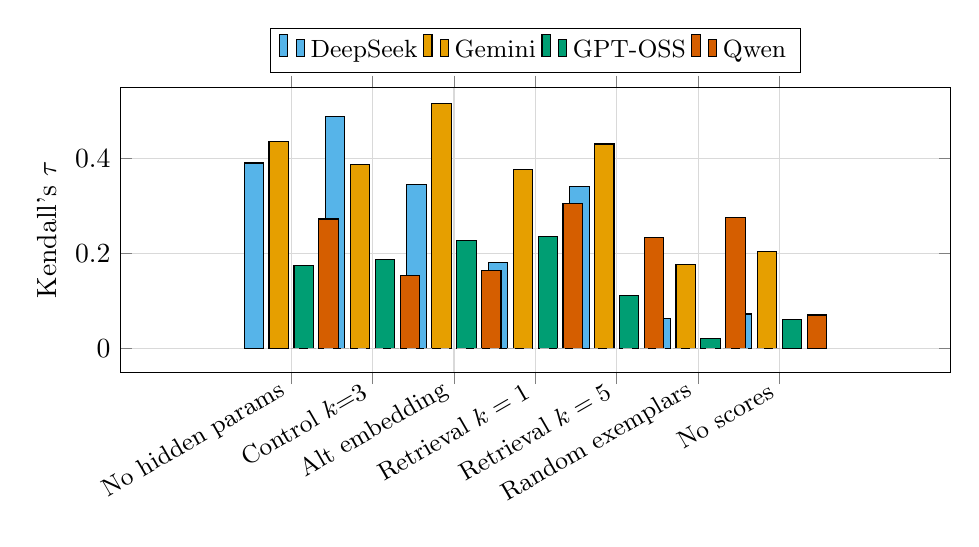
\begin{tikzpicture}
\begin{axis}[
    width=\textwidth, height=5.2cm,
    ylabel={Kendall's $\tau$},
    symbolic x coords={No hidden params,Control $k{=}3$,Alt embedding,Retrieval $k=1$,Retrieval $k=5$,Random exemplars,No scores},
    xtick=data,
    xticklabel style={rotate=30, anchor=east, font=\small, align=center},
    enlarge x limits=0.35,
    bar width=7pt,
    ybar,
    ymin=-0.05, ymax=0.55,
    legend style={font=\small, at={(0.5,1.05)}, anchor=south, legend columns=4},
    legend cell align={left},
    grid=major,
    grid style={gray!30},
    ymajorgrids=true,
]
\addplot[fill=colorDeepSeek] coordinates {
    (No hidden params,0.391)
    (Control $k{=}3$,0.489)
    (Alt embedding,0.346)
    (Retrieval $k=1$,0.182)
    (Retrieval $k=5$,0.342)
    (Random exemplars,0.063)
    (No scores,0.073)
};
\addplot[fill=colorGemini] coordinates {
    (No hidden params,0.437)
    (Control $k{=}3$,0.387)
    (Alt embedding,0.517)
    (Retrieval $k=1$,0.377)
    (Retrieval $k=5$,0.431)
    (Random exemplars,0.177)
    (No scores,0.204)
};
\addplot[fill=colorGPTOSS] coordinates {
    (No hidden params,0.175)
    (Control $k{=}3$,0.187)
    (Alt embedding,0.227)
    (Retrieval $k=1$,0.237)
    (Retrieval $k=5$,0.112)
    (Random exemplars,0.022)
    (No scores,0.061)
};
\addplot[fill=colorQwen] coordinates {
    (No hidden params,0.273)
    (Control $k{=}3$,0.154)
    (Alt embedding,0.165)
    (Retrieval $k=1$,0.306)
    (Retrieval $k=5$,0.234)
    (Random exemplars,0.276)
    (No scores,0.071)
};
\addplot[dashed, gray!60, sharp plot, update limits=false] coordinates {
    (No hidden params,0) (No scores,0)
};
\legend{DeepSeek,Gemini,GPT-OSS,Qwen}
\end{axis}
\end{tikzpicture}%
}

\newcommand{\plotAlphaSweep}{%
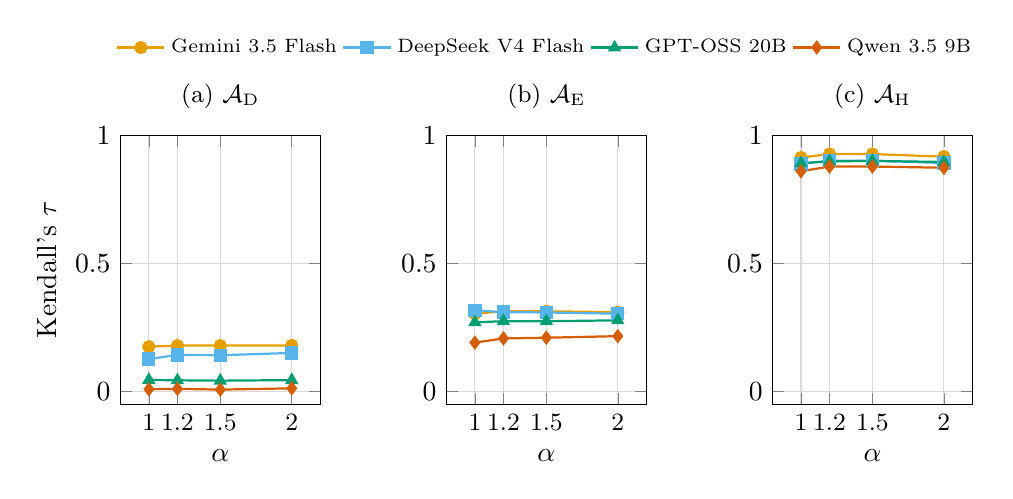
\begin{tikzpicture}
\begin{groupplot}[
    group style={group size=3 by 1, horizontal sep=1.6cm},
    width=0.34\textwidth, height=5cm,
    xlabel={$\alpha$},
    xtick={1.0,1.2,1.5,2.0},
    xticklabel style={font=\small},
    enlarge x limits=0.2,
    grid=major, grid style={gray!30}, ymajorgrids=true,
    legend style={font=\scriptsize, at={(0.5,1.25)}, anchor=south, legend columns=4, draw=none, fill=none},
    legend cell align={left},
    every axis plot/.append style={thick, mark size=2pt},
]
\nextgroupplot[ylabel={Kendall's $\tau$}, ymin=-0.05, ymax=1.0,
    title={\small (a) $\mathcal{A}_{\text{D}}$}, title style={font=\small}]
\addplot[mark=*, colorGemini]   coordinates {(1.0,0.1754) (1.2,0.1795) (1.5,0.1795) (2.0,0.1802)};
\addplot[mark=square*, colorDeepSeek] coordinates {(1.0,0.1268) (1.2,0.1433) (1.5,0.1419) (2.0,0.1509)};
\addplot[mark=triangle*, colorGPTOSS] coordinates {(1.0,0.0455) (1.2,0.0441) (1.5,0.0427) (2.0,0.0448)};
\addplot[mark=diamond*, colorQwen] coordinates {(1.0,0.0093) (1.2,0.0107) (1.5,0.0079) (2.0,0.0127)};
\nextgroupplot[ylabel={}, ymin=-0.05, ymax=1.0,
    title={\small (b) $\mathcal{A}_{\text{E}}$}, title style={font=\small}]
\addplot[mark=*, colorGemini]   coordinates {(1.0,0.3037) (1.2,0.3133) (1.5,0.3133) (2.0,0.3099)};
\addplot[mark=square*, colorDeepSeek] coordinates {(1.0,0.3169) (1.2,0.3101) (1.5,0.3087) (2.0,0.3039)};
\addplot[mark=triangle*, colorGPTOSS] coordinates {(1.0,0.2704) (1.2,0.2745) (1.5,0.2745) (2.0,0.2780)};
\addplot[mark=diamond*, colorQwen] coordinates {(1.0,0.1911) (1.2,0.2075) (1.5,0.2102) (2.0,0.2164)};
\legend{Gemini 3.5 Flash, DeepSeek V4 Flash, GPT-OSS 20B, Qwen 3.5 9B}
\nextgroupplot[ylabel={}, ymin=-0.05, ymax=1.0,
    title={\small (c) $\mathcal{A}_{\text{H}}$}, title style={font=\small}]
\addplot[mark=*, colorGemini]   coordinates {(1.0,0.9131) (1.2,0.9268) (1.5,0.9268) (2.0,0.9165)};
\addplot[mark=square*, colorDeepSeek] coordinates {(1.0,0.8884) (1.2,0.9008) (1.5,0.9008) (2.0,0.8919)};
\addplot[mark=triangle*, colorGPTOSS] coordinates {(1.0,0.8912) (1.2,0.8982) (1.5,0.8998) (2.0,0.8958)};
\addplot[mark=diamond*, colorQwen] coordinates {(1.0,0.8595) (1.2,0.8780) (1.5,0.8780) (2.0,0.8733)};
\end{groupplot}
\end{tikzpicture}%
}

% --- End inline figure definitions ---
\definecolor{colorPure}{RGB}{180,180,180}
\definecolor{colorRAG}{RGB}{100,149,200}
\definecolor{colorLLMParameterizedReferenceScoring}{RGB}{31,73,125}
\definecolor{colorGemini}{HTML}{E69F00}
\definecolor{colorDeepSeek}{HTML}{56B4E9}
\definecolor{colorGPTOSS}{HTML}{009E73}
\definecolor{colorQwen}{HTML}{D55E00}
\journal{Environmental Modelling \& Software}
\begin{document}
\begin{frontmatter}
\title{Benchmarking LLM Integration Strategies for MCDA-Assisted Household Energy Decision Support}
\author{Ahaan Nigam\corref{cor1}}
\cortext[cor1]{Corresponding author.}
\ead{ishaannigam27@gmail.com}
\affiliation{organization={Downingtown East High School},
            city={Exton},
            state={Pennsylvania},
            country={USA}}
\author{River Huang}
\affiliation{organization={Paul Scherrer Institut},
            city={Villigen},
            state={Aargau},
            country={Switzerland}}
\begin{abstract}
Everyday decisions such as setting a thermostat or scheduling an appliance can lower a household's carbon footprint, but households make them by rules of thumb. Multi-criteria decision analysis (MCDA) could optimize these decisions, but an expert must first specify how the household trades off cost, emissions, comfort and convenience. We benchmark three ways to place a large language model (LLM) inside an MCDA workflow (direct LLM scoring, example-guided LLM scoring and LLM-parameterized reference scoring) on 195 household energy scenarios with four models. In LLM-parameterized reference scoring, the LLM only extracts the engineering parameters a deterministic calculator needs. This architecture reproduces a physics-based reference ranking at Kendall's $\tau=0.880$--$0.923$ and costs the least to run, while direct LLM scoring stays near chance. LLMs should not score MCDA-based environmental recommendations themselves, but in any domain with a validated modeling calculator, an LLM can translate a plain-language description into that calculator's inputs.\end{abstract}
\begin{keyword}
Large language models \sep Multi-criteria decision analysis  \sep Household energy \sep Retrieval-augmented generation \sep Tool augmentation \sep Multi-attribute value theory \sep Sensitivity analysis
\end{keyword}
\end{frontmatter}

\section{Introduction}
\label{sec:introduction}
The average U.S.\ household emits roughly 8{,}744 pounds of CO\textsubscript{2}e and consumes about 10{,}791 kWh of electricity each year \cite{epa_household2024,eia_faq_electricity2024}. Globally, residential energy consumption has grown at roughly 1\% per year since 2000, a trend that larger homes and rising comfort demands in emerging economies have driven \cite{GONZALEZTORRES2022112428}. A considerable portion of this usage is adjustable, creating opportunities to reduce both household spending and environmental impact \cite{dietz2009}. The adjustments themselves are ordinary: a thermostat setpoint, the hour a dishwasher runs, the length of a shower. Each one trades money against emissions, comfort and convenience, and a household choosing among them has no ready way to price those four against each other.

Multi-Criteria Decision Analysis (MCDA) \cite{huang2011} addresses this kind of trade-off. Given a correctly specified value model, MCDA ranks the alternatives consistently with the decision-maker's stated preferences across all criteria at once. Building that model means defining the alternatives, criteria, weights, value functions and normalization rules, work that takes expertise and time no household will spend on a routine decision. Households' own estimates are a poor substitute: \citet{attari2010} found that people underestimate energy use and savings by a factor of 2.8 on average.

A language model can read an unstructured description of a home and a decision and return structured fields, which takes the specification work off the household. We propose three positions an LLM can occupy inside an MCDA workflow. In direct LLM scoring, the model scores each alternative on each criterion itself. In example-guided LLM scoring, the model does the same with retrieved worked examples in its prompt. In LLM-parameterized reference scoring, the model only extracts the engineering parameters that a deterministic reference calculator needs, and the calculator produces the scores. The three positions differ in the infrastructure a practitioner must maintain as well as in accuracy: direct LLM scoring needs only a prompt, example-guided LLM scoring needs an index of worked examples, and LLM-parameterized reference scoring needs a calculator. A practitioner should choose by how much accuracy each piece of infrastructure adds.

The three-way division is ours, but each position builds on an established line of work. Direct LLM scoring applies the LLM-as-judge framework that \citet{zheng2023judging} formalized, in which a model's generated scores stand in for human ratings. Example-guided LLM scoring combines retrieval-augmented generation \cite{lewis2020} with the case-based reasoning premise that a solver can reuse the solution to a similar past case \cite{aamodtplaza1994,minorkaucher2024}. LLM-parameterized reference scoring is a form of tool augmentation, which \citet{goodell2025} used to raise calculation accuracy in clinical question answering.

MCDA studies have begun to use LLMs to construct decision models or to score alternatives \cite{svoboda2024,icaart26}, but researchers have tested tool augmentation only on tasks whose correct answer does not depend on anyone's preferences, such as a numerical or factual answer \cite{gao2023pal,schick2023toolformer}, a logical conclusion \cite{pan2023logiclm}, a plan \cite{liu2023llmp} or an optimization model \cite{ramamonjison2023nl4opt,ahmaditeshnizi2024optimus}. \citet{goodell2025} gave a model task-specific clinical calculator tools and closed most of the gap to the correct answer, far beyond what retrieval alone achieved (Section~\ref{sec:lit-numeracy}). A multi-criteria ranking has no single correct number. It requires weighting incommensurable criteria against each other before any ordering exists, and a model that computes each criterion well can still order the alternatives wrongly. No prior study asks whether tool augmentation keeps its advantage through that weighting step, and none compares competing LLM-integration strategies under a shared, calculation-based standard for household energy decisions.

We make one design proposition and ask one research question:
\begin{itemize}
\item \textbf{Proposition}: An LLM can occupy three positions in an MCDA workflow: it can score the alternatives, score them with retrieved worked examples, or supply the inputs of a deterministic calculator.
\item \textbf{RQ}: How accurately does each position reproduce a deterministic reference ranking?
\end{itemize}

We test the proposition and answer the question by benchmarking the three architectures against a physics-based multi-attribute value theory (MAVT) reference across 195 household energy scenarios in three decision types: HVAC setpoints, appliance scheduling and shower duration. We hold the MAVT weights and the model access fixed across four LLMs, so the integration strategy is the only variable under test. A ranking is either right or wrong, so a badly estimated parameter matters only if it changes the alternative we recommend. We therefore report each extraction error alongside the probability that it moves the top-ranked alternative.

Our results support a division of labor. When a model reads a situation and judges it in one step, it must both understand the situation and compute the outcome, and its judgment inherits whatever scoring biases and arithmetic weaknesses the model brings to the second task. When the model only translates an unstructured description into the inputs of a validated calculator, the calculator takes over the second task.

We review research on household energy decisions, on MCDA and its automation, and on LLM numeracy and tool augmentation in Section~\ref{sec:lit-review}, and identify the gap this study fills. We define the value model, the three architectures and the evaluation procedure in Section~\ref{sec:methodology} and apply them to household energy decisions in Section~\ref{sec:experimental-design}. We report the results in Section~\ref{sec:results}, starting with non-LLM baselines that rank the alternatives without any per-scenario inference (Section~\ref{sec:res-baselines}), then interpret the results and state their limitations in Section~\ref{sec:discussion} and conclude in Section~\ref{sec:conclusion}. The objective weight vectors and the full per-model results are in Tables S2.2 and S2.16.

\section{Literature Review}
\label{sec:lit-review}
Households misjudge their own energy use by a wide margin \cite{attari2010}, and LLMs make errors in the arithmetic that turns a physical quantity into a dollar or emissions figure \cite{imani2023mathprompter}. MCDA researchers have nonetheless begun to build LLMs into their workflows, without a calculated standard that could show the output to be wrong.

\subsection{Household Energy Decision-Making and Adoption Barriers}
\label{sec:lit-barriers}

Residential buildings account for 20\% of global CO\textsubscript{2} emissions, and HVAC systems alone for roughly a third of global residential energy consumption \cite{GONZALEZTORRES2022112428}. In the United States, the residential sector consumed 19.2 quadrillion BTU (5,627 TWh) of delivered energy in 2025 and produced roughly 18\% of national energy-related CO\textsubscript{2} emissions \cite{eia_mer2026}. \citet{dietz2009} estimated that household actions could cut U.S.\ emissions by 123 MtC (about 451 MtCO\textsubscript{2}) a year within ten years, 7.4\% of U.S.\ national emissions at the time. Applying the same share to the 4{,}904 MtCO\textsubscript{2} of U.S.\ energy-related emissions in 2025 \cite{eia_co2_2025} gives a present-day potential of about 363 MtCO\textsubscript{2}. We plot residential emissions for Pennsylvania, the state in which we set this study's scenarios, in Figure~\ref{fig:pa_residential_emissions}.

\begin{figure}[htbp]
  \centering
  \includegraphics[width=0.75\textwidth]{PA_Residential_Emissions_Area.png}
  \caption{Pennsylvania residential emissions from on-site fuel combustion, by fuel, 2005--2022 (data from \citet{padep_ghg2026}).}
  \label{fig:pa_residential_emissions}
\end{figure}
%todo: ask about formatting (huang) and whether there shoud be a title

Space heating accounts for 42\% of household site energy use, followed by water heating (18\%) and air conditioning (9\%), and appliances, electronics and lighting make up most of the remaining 30\% \cite{eia_recs2020}. We cover all four through three decision types: HVAC (space heating and air conditioning), appliance scheduling, and shower duration (water heating). Which reductions households achieve depends on behavioral plasticity, the share of households not yet taking an action that effective interventions could persuade to take it. \citet{dietz2009} combine each action's plasticity with its technical potential to obtain its reasonably achievable emission reduction (RAER), and we plot all three quantities for seventeen household actions in Figure~\ref{fig:lifestyle_emissions_impact}.

\begin{figure}[H]
	\centering
	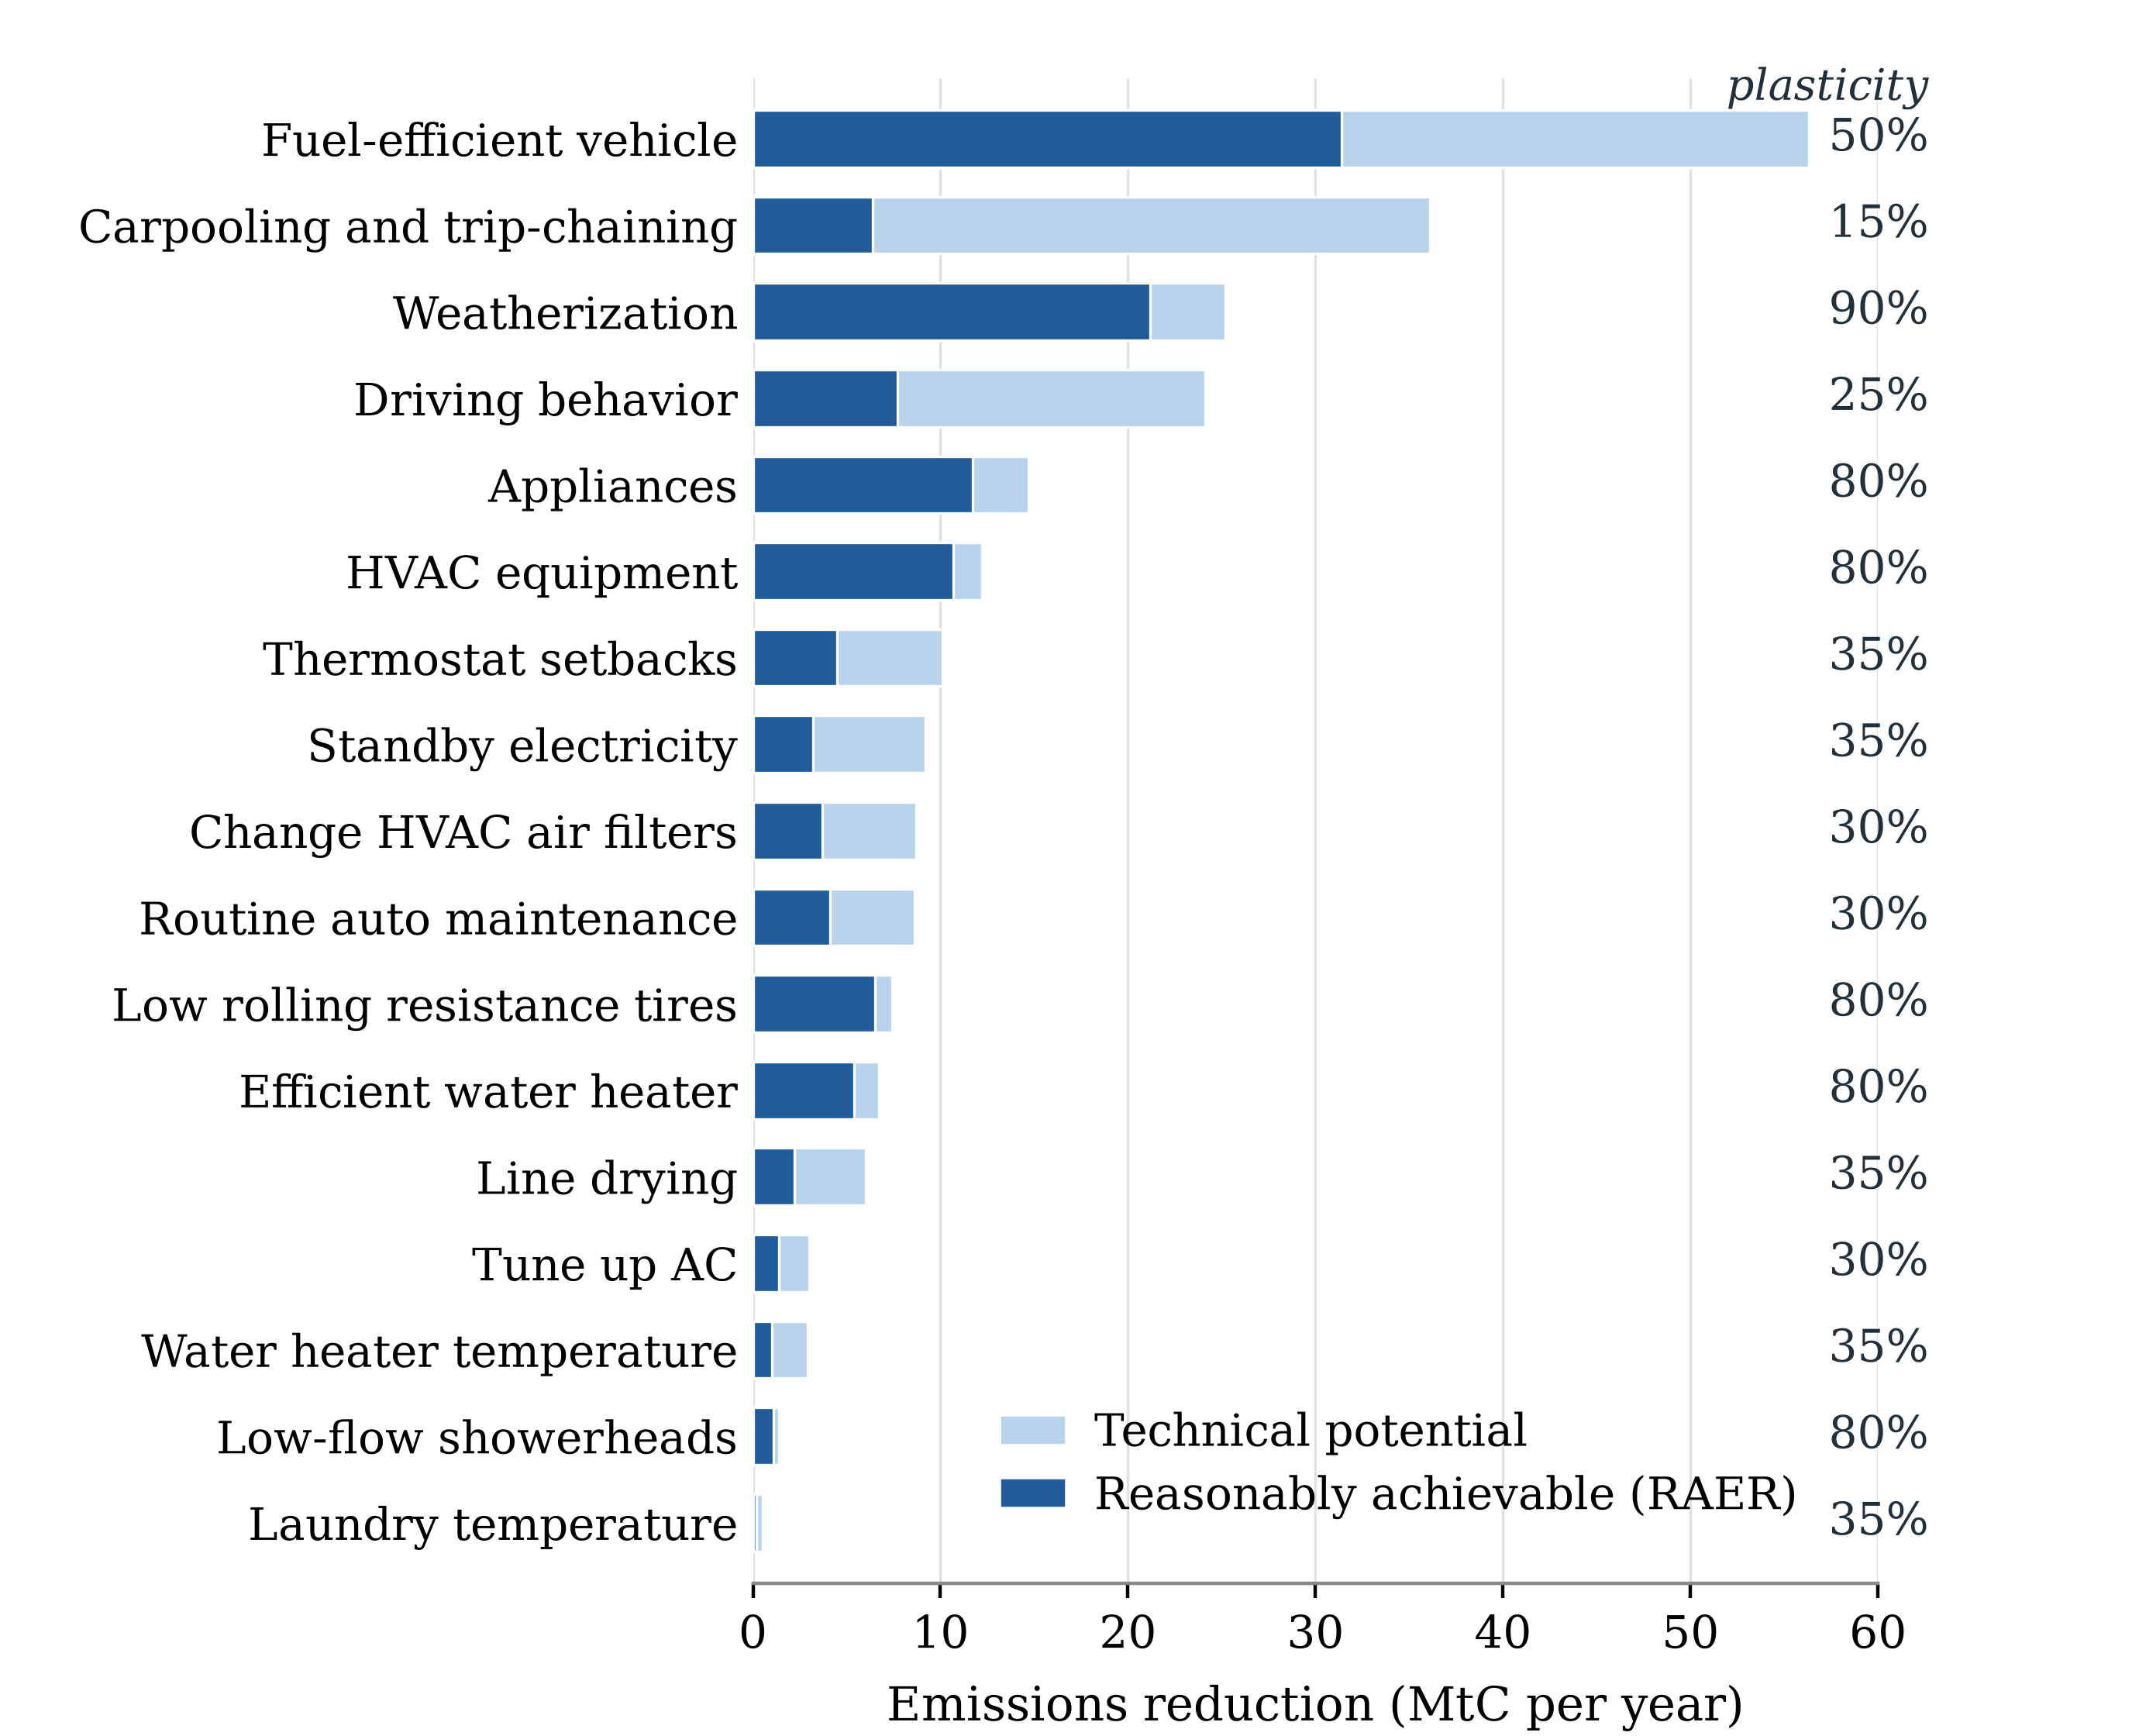
\includegraphics[width=0.8\textwidth]{LifestyleChangesEmissionImpact.png}
\caption{Emission-reduction potential of household actions (data from \citet{dietz2009}, Table~1).}
\label{fig:lifestyle_emissions_impact}
\end{figure}

Households misjudge their energy use in a systematic way: they underestimate the energy that high-consumption activities draw and overestimate it for low-consumption ones \cite{attari2010}. A household therefore chooses its usual thermostat setpoint, appliance run time or shower length on wrong or arbitrary assumptions. Even with a streamlined MCDA calculator \cite{huangburgherr2024}, the user must still frame the alternatives, criteria and weights, which takes more time and effort than a household will spend on a routine decision.

Heuristic routines let households resolve everyday decisions quickly, but in laboratory choice tasks some of these heuristics break down under time pressure \cite{bobadilla2018}, and households fall back on satisficing: choosing the first acceptable option instead of weighing trade-offs. Status quo bias keeps households at their habitual level of energy use even when changing it would save money \cite{gill2022}. A decision-support tool adds steps to a decision the household used to make by habit, so its designer has to keep that added effort small. Explanations help: \citet{sardianos2021} found that a recommender that set out the financial savings and environmental benefit behind each suggestion raised user acceptance by 19\%.

\subsection{MCDA and Its Automation}
\label{sec:lit-mcda}

An MCDA problem specifies a finite set of alternatives evaluated against multiple criteria, each carrying a weight that reflects its relative importance to the decision-maker. The formalization originates in classical decision theory \cite{keeneyraiffa1976,dyer1979}. The classical toolkit spans several method families beyond MAVT: the Analytic Hierarchy Process (AHP) derives weights from pairwise comparisons, the Technique for Order of Preference by Similarity to Ideal Solution (TOPSIS) ranks alternatives by distance from an ideal and an anti-ideal point, and outranking methods such as ELECTRE and PROMETHEE compare alternatives pairwise without collapsing them into a single index \cite{huang2011}.

MAVT combines single-attribute value functions into one score using criterion weights. Those weights reflect the intended trade-offs only when the decision-maker sets them with the attribute ranges of the choice set in view \cite{vonnitzsch1993}. Fuzzy variants such as fuzzy AHP and fuzzy TOPSIS address a related problem, imprecise judgments, by representing them with fuzzy sets \cite{zadeh1965} rather than crisp weights.

Recent studies use LLMs to elicit preferences, generate alternatives or score alternatives directly \cite{svoboda2024,icaart26}, and \citet{vahidnia2025walmas} go further, asking a multi-agent LLM panel to assign the criterion weights. None of these studies checks the output against an independently computed answer. \citet{svoboda2024} report a consistency ratio within threshold, \citet{icaart26} report improved ranking consistency, and \citet{anhao2025probid} report fuzzy membership scores with no external check, so each study validates the procedure rather than the answer.

We summarize the studies that have placed an LLM inside an MCDA workflow in Table~\ref{tab:llm-mcda-prior-work}. Four of the five LLM-integrated studies report no ground truth; the exception, \citet{cheng2026wildfire}, compares LLM-generated criterion weights with expert-assigned weights from a published study. None of the five checks a ranking of alternatives against a calculated standard.

\begin{table}[htbp]
\caption{Prior LLM--MCDA integration studies.}
\label{tab:llm-mcda-prior-work}
\centering
\begin{threeparttable}
\centering
\footnotesize
\begin{tabular}{@{}>{\raggedright\arraybackslash}p{0.15\textwidth}>{\raggedright\arraybackslash}p{0.16\textwidth}>{\raggedright\arraybackslash}p{0.40\textwidth}p{0.13\textwidth}@{}}
\toprule
\textbf{Study} & \textbf{MCDA method} & \textbf{LLM's role} & \textbf{Ground truth?} \\
\midrule
\citet{svoboda2024} & AHP & GPT-4 agents act as virtual experts generating pairwise comparisons & No \\
\citet{icaart26} & COMET & LLaMA 3.1 8B substitutes for the human expert who scores characteristic objects & No \\
\citet{cheng2026wildfire} & AHP & Five LLMs generate criterion weights under four prompting strategies (direct, multi-model debate, full-document, indicator-guided) & Yes\tnote{a} \\
\citet{vahidnia2025walmas} & Weight elicitation & Multi-agent LLMs substitute for an expert panel assigning criterion weights & No\tnote{b} \\
\citet{anhao2025probid} & Fuzzy PROBID & LLM semantic-similarity judgments generate fuzzy membership scores & No \\
\citet{huangburgherr2024} & Multi-method DSS & None (conventional expert-elicited inputs) & N/A \\
\bottomrule
\end{tabular}
\begin{tablenotes}
\item[a] Expert-assigned criterion weights from one published study.
\item[b] Inter-agent agreement (Kendall's W) and IQR outlier removal across the LLM panel.
\end{tablenotes}
\end{threeparttable}
\end{table}

\subsection{LLM Numeracy and Tool Augmentation}
\label{sec:lit-numeracy}

LLMs make a calculated standard hard to meet for reasons unrelated to the MCDA method around them. Their outputs change with prompt formatting that carries no meaning \cite{sclar2024promptsensitivity}. \citet{zheng2023judging} formalized the LLM-as-judge framework, in which a model's generated scores stand in for human ratings; \citet{wang2024fairescalers} showed that such judges favor a response for its position, ranking a candidate higher for where it appears rather than for its content, and \citet{li2026scoringbias} documented scoring biases in LLM-as-a-judge pipelines that persist in advanced models. On arithmetic, LLMs often return wrong answers unless they check themselves against several generated solution paths \cite{imani2023mathprompter}.

Worked examples offer a second route to accuracy. In few-shot prompting, the prompt includes solved examples similar to the target problem. Retrieval-augmented generation (RAG) selects those examples from an external store; \citet{lewis2020} introduced it to reduce hallucination in open-domain question answering. The approach suits MCDA scoring because it mirrors case-based reasoning, which solves a new problem by retrieving similar past cases and reusing their recorded solutions \cite{aamodtplaza1994}. \citet{minorkaucher2024} found that retrieved example explanations, used as in-context demonstrations, improve LLM outputs over zero-shot prompting.

A third route removes the scoring from the model's task: the model translates natural language into the inputs of an external tool, and the tool does the calculation. The model can write a program for an interpreter to run \cite{gao2023pal}, call a calculator or search engine it has learned to use \cite{schick2023toolformer}, or state a problem formally for a logic solver \cite{pan2023logiclm}, a classical planner \cite{liu2023llmp} or an optimization solver \cite{ramamonjison2023nl4opt,ahmaditeshnizi2024optimus}. In building energy modeling, EPlus-LLM translates a natural-language description of a building into an EnergyPlus input file and cuts modeling effort by over 95\% \cite{jiang2024eplus}. \citet{zhang2025agentic} built an agentic workflow in which the LLM extracts the model's objects from a building description and repairs them against EnergyPlus's own error reports. \citet{goodell2025} compared a base model, a retrieval-augmented model and a model given task-specific clinical calculator tools, among five configurations they ran across 10{,}000 trials of medical calculation questions: accuracy rose from 11.4\% to 40.3\% to 84.0\% on LLaMa-3.1-70b and from 36.1\% to 76.8\% to 95.2\% on GPT-4o.

Every task in that comparison has one correct number, and an MCDA ranking does not. Before any ordering exists, the method weights and aggregates the criterion estimates, and an error that is small on one criterion can still reverse the order of two alternatives. We ask whether tool augmentation keeps its advantage when the model's output must pass through that weighting and aggregation before it becomes a decision.

\section{Methodology}
\label{sec:methodology}

We describe the evaluation framework without reference to any application domain, so that it applies to any decision for which a validated calculator exists. Below we define the multi-attribute value model that produces the reference ranking (Section~\ref{sec:mavt-design}), describe three ways to place a language model in the decision workflow (Section~\ref{sec:architectures}), and set out the metrics and statistical tests we use to compare them (Section~\ref{sec:eval-metrics}). We apply the framework to household energy decisions in Section~\ref{sec:experimental-design}. The notation is in Table S1.1.

\subsection{MAVT Formulation}
\label{sec:mavt-design}
MAVT scores each alternative on every criterion, converts each score to a common 0--1 value scale, and combines the values into a single weighted score \cite{keeneyraiffa1976,dyer1979}. The additive form (Eq.~\ref{eq:mavt_sum}) is valid when the criteria are mutually preferentially independent \cite{keeneyraiffa1976,dyer1979}. A subset of criteria is preferentially independent of the remaining criteria when the decision-maker's preferences among outcomes that differ only on that subset do not depend on the levels of the remaining criteria; mutual preferential independence requires this of every subset. The condition concerns the decision-maker's preferences, not the data: two criteria can be highly correlated across a set of alternatives and still be preferentially independent (Section~\ref{sec:criteria-weighting}).

\begin{equation}
\label{eq:mavt_sum}
s_j = \sum_{i=1}^{4} w_i \cdot v_i(x_{ij})
\end{equation}

\noindent where $s_j$ is the aggregate score of alternative $j$, $w_i$ the weight of criterion $i$, $x_{ij}$ the raw value of alternative $j$ on criterion $i$, and $v_i$ that criterion's value function.

We first convert each criterion's raw quantity $x$ to a normalized value $\tilde{x}$ against a fixed reference range $[x_{\min}, x_{\max}]$ for that criterion (ranges in Section~\ref{sec:gt-calculators}), oriented so that higher values are always better:

\begin{equation}
\label{eq:norm_x}
\tilde{x} =
\begin{cases}
\dfrac{x - x_{\min}}{x_{\max} - x_{\min}} & \text{for increasing criteria}\\[4mm]
\dfrac{x_{\max} - x}{x_{\max} - x_{\min}} & \text{for decreasing criteria}
\end{cases}
\end{equation}

A criterion on which equal changes in the raw quantity are equally valuable takes the linear value function (Eq.~\ref{eq:linear_vf}) \cite{dyer1979,keeneyraiffa1976}.

\begin{equation}
\label{eq:linear_vf}
v_i(\tilde{x}) = \tilde{x}
\end{equation}

A criterion with diminishing marginal returns takes the logarithmic value function (Eq.~\ref{eq:log_vf}): an improvement from a poor starting point is worth more to the decision-maker than the same improvement near the optimum. The shape parameter $\alpha$ sets the curvature, and a larger $\alpha$ gives stronger diminishing returns.

\begin{equation}
\label{eq:log_vf}
v_i(\tilde{x}) = \frac{\ln\!\left(1 + \alpha \cdot \tilde{x}\right)}{\ln(1 + \alpha)}
\end{equation}

\FloatBarrier
\subsection{Integration Architectures}
\label{sec:architectures}

We compare three ways of placing a language model inside an MCDA workflow: direct LLM scoring ($\mathcal{A}_{\text{D}}$), example-guided LLM scoring ($\mathcal{A}_{\text{E}}$), and LLM-parameterized reference scoring ($\mathcal{A}_{\text{H}}$). We hold every other design choice fixed, including the model, the criterion weights and the set of scenarios.

In direct LLM scoring, the model does the whole job. For each alternative, the model returns a score on every criterion, and we rank the alternatives by their MAVT aggregate (Eq.~\ref{eq:mavt_sum}). We give the model an analyst role and structured-output constraints \cite{icaart26}, instruct it to make a reasonable estimate when a detail is missing, and supply no information beyond the description of the situation. Because the model does all of the scoring, $\mathcal{A}_{\text{D}}$ needs only a prompt and access to a model, which makes it the simplest of the three to implement.

Example-guided LLM scoring adds a retrieval step, following the retrieval-augmented generation pattern \cite{lewis2020}. Before scoring, the system retrieves the most similar previously solved case from an index and shows it to the model as a worked example: the case's descriptive attributes, the engineering parameters behind its physical evaluation, and, for each of its alternatives, the criterion scores, aggregate score and rank that the reference calculator produced. We instruct the model to treat the example as a reference point and to score the current situation on its own merits rather than copy the example's scores. On top of everything $\mathcal{A}_{\text{D}}$ requires, $\mathcal{A}_{\text{E}}$ needs a searchable set of solved cases and the infrastructure to index and query them.

In LLM-parameterized reference scoring, we do not ask the model for scores. We ask it instead to estimate the engineering parameters that the situation description leaves out, values a homeowner would not know or report. We pass every other input, including the attributes the description does report and the list of alternatives, directly to a deterministic calculator, which converts the full parameter set into criterion scores and an aggregate. The model's role shrinks to filling in what the calculator cannot observe. We diagram the steps of each architecture in Figure~\ref{fig:pipeline}.

\begin{figure}[H]
	\centering
	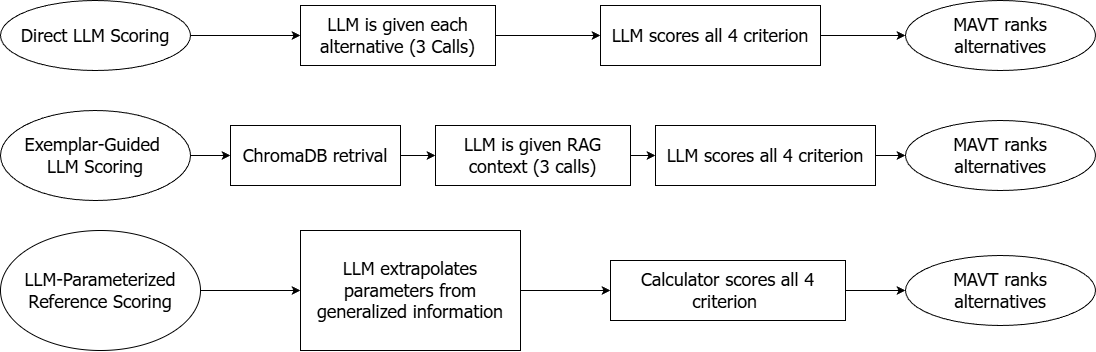
\includegraphics[width=1\textwidth]{ArchitectureFlowcharts.png}
  \caption{Processing steps of the three integration architectures.}
\label{fig:pipeline}
\end{figure}

In this study, $\mathcal{A}_{\text{H}}$ calls the same calculator that produces the reference scores. We measure how much of its accuracy that access alone provides in Section~\ref{sec:res-baselines}, explain in Section~\ref{sec:interpretation} why most extraction errors leave the ranking unchanged, and set out in Section~\ref{sec:limitations} what grading an architecture against its own calculator can and cannot show.

\subsection{Evaluation Metrics}
\label{sec:eval-metrics}
We evaluate accuracy on both scores and rankings. Environmental modelling guidance recommends choosing performance criteria to fit the model's purpose and combining several of them rather than relying on one \cite{jakeman2006tensteps,bennett2013characterising}. For score error, we compute the mean absolute error (MAE) and root mean squared error (RMSE) between an architecture's scores and the reference scores on the 0--1 MAVT scale, for each criterion and then across criteria. For ranking accuracy, we compute Kendall's $\tau$ between the architecture's ranking of the three alternatives and the reference ranking, and Top-1 accuracy, the share of scenarios in which the architecture's top-ranked alternative is also the reference's. We average per-scenario values across the 195 test scenarios. With $n=3$ alternatives, each scenario contains three pairwise comparisons, so a scenario's $\tau$ can take only the values $-1$, $-\frac{1}{3}$, $\frac{1}{3}$ and $1$, according to whether none, one, two or all three pairs are in the correct order. We break exact ties in the aggregate score by a fixed criterion priority (Environmental Impact, then Energy Cost, Comfort and Practicality) and, if alternatives remain tied, by input order (Section~\ref{sec:models-implementation}). Every ranking is therefore strict, so an averaged $\tau$ converts exactly into the share of pairwise comparisons in the correct order, $(1+\tau)/2$. A uniformly random ranking gives Top-1 accuracy of $1/3$ and an expected $\tau$ of 0, which corresponds to half the pairs in the correct order.

We call a difference significant when a paired test rejects, at the 0.05 level after Holm correction within its family of comparisons, the hypothesis that the two systems under comparison rank the scenarios equally well. A significant difference can still be too small to matter, so we report effect sizes and confidence intervals with each test. We measure efficiency by total tokens (input plus output) and API cost, each summed over the 195-scenario test set, and we compute the run-to-run standard deviation of each metric, treating runs rather than scenarios as the unit of analysis. A scenario fails when we cannot parse the model's response or the response contains a value outside its valid range, and the pipeline then records a reserved sentinel value. We compute accuracy metrics on successful scenarios only and count failures separately. Exclusion applies per model, architecture and run, so a scenario that fails in one run still counts in the runs where it succeeded. $\mathcal{A}_{\text{D}}$ and $\mathcal{A}_{\text{E}}$ make one call per alternative and fail the whole scenario if any call fails, while $\mathcal{A}_{\text{H}}$ makes a single extraction call per scenario. Because failure rates differ across models and architectures, we report the failure counts and a success-weighted correction in Section~\ref{sec:res-ranking}, and in Table S2.13 we repeat the analysis with each failed score set to the 0.5 scale midpoint.

We compare architectures with paired Wilcoxon signed-rank tests that take the scenario as the unit of analysis. For each scenario, we average the metric over the runs in which that scenario succeeded, five for most scenarios and fewer where a run failed. Our paired bootstrap confidence intervals resample scenarios and keep all successful runs of a drawn scenario together. We Holm-correct the Wilcoxon tests of the main architecture comparison as a single family (enumerated in Supplementary Material S2), and we never pool models.

We test the ablations of Section~\ref{sec:ablation-design} in two stages. Where an ablation compares more than two configurations, we first run a Friedman test of whether any configuration differs from the others. If none does, we report the set as indistinguishable and stop; if one does, we compare the configurations pairwise with Wilcoxon signed-rank tests. We Holm-correct the omnibus tests and the pairwise tests as two separate families, so running many comparisons cannot by itself produce a significant result. For each significant pair we report Cliff's $\delta$ as the effect size, and we compute percentile bootstrap 95\% confidence intervals for every configuration whether or not its omnibus test reached significance. A comparison of exactly two conditions skips the omnibus stage. The test families are in Supplementary Material S2.


\FloatBarrier

\section{Experimental Design}
\label{sec:experimental-design}

We apply the framework of Section~\ref{sec:methodology} to three household decisions: where to set a thermostat, when to run an appliance and how long to shower.

\subsection{Decision Types and Scenario Dataset}
\label{sec:dataset}
We gave HVAC the most scenarios because it carries the largest share of residential energy use, a share that grows with rising comfort demands (Section~\ref{sec:lit-barriers}). Appliance and Shower received fewer because they have fewer categorical inputs to combine: an Appliance scenario varies the appliance, its age and the housing type, and a Shower scenario only the flow-rate tier and the housing type, so fewer scenarios cover their realistic combinations. The test set contains 195 scenarios (70 HVAC, 65 Appliance and 60 Shower), each with three alternatives that every architecture and the reference calculator score independently. A separate RAG set of 90 scenarios (35 HVAC, 35 Appliance and 20 Shower) populates the retrieval index of $\mathcal{A}_{\text{E}}$ \cite{lewis2020} and never enters evaluation (Supplementary Material S1). We drew both sets from one audited scenario matrix that covers realistic combinations of the categorical inputs, from a poorly insulated rowhouse to a well-insulated apartment, and kept the two sets fully disjoint. We trace how the 285 scenarios divide between the two sets, and how each set reaches the reference calculators and the three architectures, in Figure S1.1.

In the test scenarios, we withhold each scenario's exact engineering parameters (R-value, SEER, HVAC equipment age and occupancy context for HVAC; kWh per cycle for Appliance, whose type and baseline run time appear only in the question's free text; GPM, tank size and heater setpoint for Shower) and show homeowner-accessible information in their place, such as an insulation tier instead of an R-value. A function derives each label from the scenario's raw value, so the architectures see what a homeowner could report while the reference calculator uses what the physics requires. The retrieved RAG exemplars, by contrast, include their own engineering values as part of the worked example (Section~\ref{sec:architectures}). We mark which parameters the LLMs and the calculators receive for each decision type in Table~\ref{tab:parameter_comparison}. Every field's observed range, the label bands and their governing standards, the insulation and SEER tiers, and the housing-type mappings are in Tables S1.2 and S1.3.

\begin{table}[htbp]
\caption{Parameters received by the LLMs and by the reference calculators.}
\label{tab:parameter_comparison}
\centering
\footnotesize
\renewcommand{\arraystretch}{0.88}
\setlength{\tabcolsep}{3pt}
\begin{minipage}[t]{0.31\textwidth}\vspace{0pt}
\centering
\textbf{HVAC}\\[0.3em]
\begin{tabular}{@{} l c c @{}}
\toprule
\textbf{Parameter} & \textbf{LLMs} & \textbf{Calc.} \\
\midrule
Location            & \checkmark & ---        \\
Outdoor Temp        & \checkmark & \checkmark \\
Home Size (sq ft)   & \checkmark & \checkmark \\
Insulation Tier$^{a}$   & \checkmark & ---        \\
R-Value             & ---        & \checkmark \\
Household Size      & \checkmark & \checkmark \\
Housing Type        & \checkmark & \checkmark \\
House Age$^{b}$     & \checkmark & ---        \\
Utility Budget      & \checkmark & \checkmark \\
SEER Rating         & ---        & \checkmark \\
HVAC Age            & ---        & \checkmark \\
Occupancy Context$^{c}$   & \checkmark & \checkmark \\
Indoor Temp (alt.)  & A          & \checkmark \\
\bottomrule
\end{tabular}
\end{minipage}%
\hfill
\begin{minipage}[t]{0.31\textwidth}\vspace{0pt}
\centering
\renewcommand{\arraystretch}{1.04}
\textbf{Appliance}\\[0.3em]
\begin{tabular}{@{} l c c @{}}
\toprule
\textbf{Parameter} & \textbf{LLMs} & \textbf{Calc.} \\
\midrule
Appliance Type          & T          & \checkmark \\
Baseline Runtime        & T          & \checkmark \\
Appliance Age Tier      & \checkmark & ---        \\
kWh per Cycle           & ---        & \checkmark \\
TOU Period / Utility Rate & ---      & \checkmark \\
Monthly Cycles          & ---        & \checkmark \\
Household Size          & \checkmark & \checkmark \\
Housing Type            & \checkmark & \checkmark \\
Location                & \checkmark & \checkmark \\
Utility Budget          & \checkmark & \checkmark \\
\bottomrule
\end{tabular}
\end{minipage}%
\hfill
\begin{minipage}[t]{0.31\textwidth}\vspace{0pt}
\centering
\renewcommand{\arraystretch}{0.955}
\textbf{Shower}\\[0.3em]
\begin{tabular}{@{} l c c @{}}
\toprule
\textbf{Parameter} & \textbf{LLMs} & \textbf{Calc.} \\
\midrule
Location                 & \checkmark & \checkmark  \\
Outdoor Temp             & \checkmark & \checkmark  \\
Inlet Water Temp         & ---        & \checkmark  \\
Heater Setpoint          & ---        & \checkmark  \\
Flow Rate Tier           & \checkmark & ---         \\
GPM                      & ---        & \checkmark  \\
Duration (min)           & A          & \checkmark  \\
Household Size           & \checkmark & \checkmark  \\
Tank Size                & ---        & \checkmark  \\
Utility Budget           & \checkmark & \checkmark  \\
Housing Type             & \checkmark & \checkmark  \\
\bottomrule
\end{tabular}
\end{minipage}
\vspace{1em}
\par{\footnotesize $^{a}$Tier labels (Poor/Medium/Good) map to R-value ranges (Supplementary Material S1).
$^{b}$LLMs receive a building-age range label (e.g., ``21--30 years''); the calculator does not use house age but uses the exact HVAC equipment age, which the LLMs do not receive.
$^{c}$The question's wording conveys occupancy.
T = free-text input; A = inferred from alternative.}
\end{table}

\FloatBarrier
\subsection{Criteria and Weighting}
\label{sec:criteria-weighting}
We weight the criteria Environmental Impact 35\%, Energy Cost 30\%, Comfort 20\% and Practicality 15\% (Table~\ref{tab:item3}) and hold the weights constant across decision types, architectures and the reference calculator. We derive objective weight vectors by entropy and by MEREC (Method based on the Removal Effects of Criteria) \cite{merec2021} in Supplementary Material S2, and we report results under those vectors and under equal weights in Section~\ref{sec:res-sensitivity}.

\begin{table}[htbp]
\caption{MAVT criterion specification.}
\label{tab:item3}
\centering
\begin{threeparttable}
\centering
\footnotesize
\renewcommand{\arraystretch}{1.15}
\begin{tabular}{lllll}
\toprule
Criterion & Weight (\%) & Value Function & $\alpha$ & Direction \\
\midrule
Environmental Impact & 35 & Linear (Eq.~\ref{eq:linear_vf}) & \textemdash & Lower raw = better \\
Energy Cost & 30 & Linear (Eq.~\ref{eq:linear_vf}) & \textemdash & Lower raw = better \\
Comfort & 20 & Logarithmic (Eq.~\ref{eq:log_vf}) & 1.5 & Higher raw = better \\
Practicality & 15 & Logarithmic (Eq.~\ref{eq:log_vf}) & 1.2 & Higher raw = better \\
\bottomrule
\end{tabular}
\renewcommand{\arraystretch}{1.0}
\end{threeparttable}
\end{table}

We weight Environmental Impact at 0.35 because the household sector produces a large share of national CO\textsubscript{2} emissions \cite{dietz2009} and because value--belief--norm theory identifies environmental orientation as a normative driver of pro-environmental behavior \cite{stern1999}. Entropy weighting of the scenario distributions independently assigns this criterion a high weight (Table S2.2). We weight Energy Cost at 0.30 for two reasons. Cost information steers household appliance purchases more than energy or emissions information does \cite{newell2014}, so a criterion set that underweights it would recommend alternatives the household would decline. Households also misjudge the energy use that drives cost (Section~\ref{sec:lit-barriers}), so an external calculation adds value there. We place Energy Cost below Environmental Impact because we built this integration to reduce environmental impact.

We weight Comfort at 0.20 because thermal comfort preferences drive residential energy use \cite{sintov2019}. We measure HVAC Comfort against ASHRAE\,55 setpoints \cite{ashrae55_2020}. For appliances, the Comfort curve follows demand-response research on how long households tolerate a scheduling delay \cite{paetz2012,waseem2020}; for showers, it peaks near the average shower duration reported in the \textit{Residential End Uses of Water, Version~2} study \cite{reu2016} and penalizes heater setpoints below the CDC's \textit{Legionella} threshold \cite{cdc2026}. Practicality, at 0.15, measures whether a household could keep repeating an alternative, which differs from whether it would choose the alternative once: friction shows up as low adoption over months rather than as discomfort on the day. A 20-minute shower at 2.5\,GPM in a four-person household with a 50-gallon tank, for example, needs about 155 gallons of hot water against the roughly 40 gallons the tank can usefully supply, so the household runs out. Comfort does not register that shortfall, so we score it under Practicality.

Energy Cost and Environmental Impact enter the MAVT normalization as physical quantities: dollars, and pounds of CO\textsubscript{2} or gallons of water. Comfort and Practicality have no physical unit, so the calculators compute them on a bounded 0--1 scale, and the same normalization (Eq.~\ref{eq:norm_x}) maps that scale onto the constructed bounds of Table~\ref{table:reference_ranges}. Energy Cost and Environmental Impact take the linear value function; Comfort and Practicality show diminishing marginal returns and take the logarithmic one (Section~\ref{sec:mavt-design}). We set $\alpha = 1.5$ for Comfort and $\alpha = 1.2$ for Practicality a priori to introduce mild concavity, adjusting them only to keep values inside the 0--1 range; we neither elicited nor fitted either value. The architecture ordering does not change across an $\alpha$ sweep (Section~\ref{sec:res-sensitivity}).

Energy Cost and Environmental Impact are strongly correlated in this dataset: Spearman's $\rho$ between them across the 195 test scenarios is 0.92. The correlation does not violate preferential independence, which concerns the household's preferences rather than the data (Section~\ref{sec:mavt-design}). The condition requires, for example, that a household that prefers the cheaper of two alternatives equal on emissions, Comfort and Practicality prefers it at whatever levels those three criteria take, and we assume this holds for all four criteria \cite{keeneyraiffa1976,dyer1979}. The correlation does raise a redundancy concern: if the two criteria measure one underlying quantity under two names, their combined 65\% weight counts that quantity twice \cite{keeneyraiffa1976}. A double count of this kind changes what the reference recommends but favors no architecture, because we score every architecture against the same weighted reference. Moving weight off these two criteria also leaves LLM-parameterized reference scoring ahead of example-guided LLM scoring in all 20 model--weight-vector cells (Section~\ref{sec:res-sensitivity}). How far the two criteria separate depends on the decision type.

On Appliance the two criteria separate. The utility's time-of-use window sets the price period (for PECO, 2--6\,p.m.\ on weekdays \cite{peco2021}), while the PJM system-wide peak of 7\,a.m.--11\,p.m.\ sets the emissions period, so a cycle run at 8\,a.m.\ is off-peak for cost and on-peak for emissions. The two separate here because the appliance decision is itself a choice of when to run, so its alternatives can fall in different price and emissions periods. We evaluate all three alternatives of an HVAC scenario at a single time, so their cost and emissions both scale with the same energy use and move together on any grid. The three alternatives of a Shower scenario differ only in duration, and cost and water volume both scale with duration, so those two criteria move together as well. Only alternatives that draw energy at different times can separate the two criteria, which is why they separate on Appliance alone (Section~\ref{sec:limitations}).

\FloatBarrier
\subsection{Reference Calculators}
\label{sec:gt-calculators}

Each decision type has its own deterministic calculator. The three calculators share the four criteria, the value functions, the budget penalty and the emissions accounting. We give the HVAC calculator in full as the representative case, since it is the most involved of the three and uses every part of that shared frame. We outline the Appliance and Shower calculators here and give their monthly-cost conversions, rate tables and parameter bands in Supplementary Material S1; all three implementations are in the released code.

Each reference calculator takes a scenario with three alternatives and returns four scores per alternative, together with the raw Energy Cost and Environmental Impact quantities before the value functions apply. We express energy cost in dollars per 8-hour decision period (HVAC), per cycle (Appliance) or per shower (Shower), and environmental impact in pounds of CO\textsubscript{2} (HVAC and Appliance) or gallons of water (Shower). The calculators estimate monthly cost only for the budget penalty.

For each criterion and decision type, we set the raw values that the MAVT normalization (Eq.~\ref{eq:norm_x}) maps to 0 and to 1 (Table~\ref{table:reference_ranges}). For Energy Cost and Environmental Impact, these endpoints are the 5th and 95th percentiles of the scenario set's own distribution rather than of national data. We built the scenarios to represent Pennsylvania households, so their distribution serves as a proxy for Pennsylvania's, and national endpoints would compress this study's scores into a narrow part of the 0--1 scale. Comfort and Practicality have no measurable physical quantity whose distribution could supply percentiles, so we give them constructed bounds of 0.0--1.0 and 0.05--1.0. We set the Practicality floor at 0.05 because no household alternative is impossible to execute, only inadvisable.

\begin{table}[htbp]
\caption{MAVT normalization bounds by criterion and decision type.}
\label{table:reference_ranges}
\centering
\begin{threeparttable}
\centering
\small
\begin{tabular}{@{}lccc@{}}
\toprule
\textbf{Criterion} & \textbf{HVAC} & \textbf{Appliance} & \textbf{Shower} \\
\midrule
Energy Cost & 0.38--3.29 & 0.025--0.71 & 0.14--1.14 \\
Environmental Impact & 1.96--18.04 & 0.288--3.643 & 6.0--45.0 \\
Comfort & 0.0--1.0 & 0.0--1.0 & 0.0--1.0 \\
Practicality & 0.05--1.0 & 0.05--1.0 & 0.05--1.0 \\
\bottomrule
\end{tabular}
\end{threeparttable}
\end{table}
The HVAC cost percentiles are only from active-conditioning alternatives. We price electricity at a bundled Pennsylvania retail rate of \$0.19/kWh. EIA reports a lower state average of about \$0.177/kWh \cite{eia_epa_2024}, but that figure is the average revenue per kWh across all residential customers in the state, including those on legacy supply contracts. Our rate is the all-in amount a household on default service pays at the margin: generation supply plus transmission, distribution, and the customer-assistance and energy-efficiency riders that appear as separate line items on the bill, priced against the default-service rates of the six Pennsylvania utilities we model \cite{paupc2025}. At this rate, the 5th and 95th percentiles of the 8-hour cost of active-conditioning alternatives are \$0.38 and \$3.29, and an Off alternative, at zero cost, receives the top Energy Cost score. Converting the same kWh range with the PJM marginal emissions factors (0.976 lbs CO\textsubscript{2}/kWh off-peak, 1.041 peak) gives HVAC Environmental Impact bounds of 1.96--18.04 lbs CO\textsubscript{2} \cite{pjm2022emissions}.

For HVAC and Appliance, we compute Environmental Impact with PJM marginal emissions factors:
\begin{equation}
\begin{gathered}
  \mathrm{CO_2} = E_{\mathrm{kWh}} \cdot \varepsilon(t), \\[4pt]
  \varepsilon(t) = \begin{cases}
    1.041 \text{ lbs/kWh} & \text{peak (7am--11pm)} \\
    0.976 \text{ lbs/kWh} & \text{off-peak}
  \end{cases}
\end{gathered}
  \label{eq:emissions}
\end{equation}
\noindent where $E_{\mathrm{kWh}}$ is the decision-period energy use and $\varepsilon(t)$ is the PJM marginal emissions factor at run time $t$ \cite{pjm2022emissions}. We use marginal rather than average factors because shifting a residential load changes the output of the marginal generator.
All three calculators apply an identical four-tier budget penalty $P(u)$ multiplicatively to the energy-cost value-function output, where $u = C_{\mathrm{monthly}} / B$ is monthly cost utilization relative to the household's stated budget $B$:
\begin{equation}
  P(u) = \begin{cases}
    1.0                          & u < 0.80                   \\[4pt]
    1 - 2.5\,(u - 0.80)         & 0.80 \le u < 1.0           \\[4pt]
    0.5\,e^{-3(u - 1.0)}        & 1.0 \phantom{0}\le u < 1.5 \\[4pt]
    0                            & u \ge 1.5
  \end{cases}
  \label{eq:budget_penalty}
\end{equation}
\noindent where $P(u)$ is a unitless multiplicative penalty on the (post value-function) energy-cost score, $u$ is monthly budget utilization, $C_{\mathrm{monthly}}$ is estimated monthly energy/water-related cost for the decision type, and $B$ is the household-stated monthly budget for utilities.
\noindent We took only the curve's shape from the behavioral-economics literature \cite{thaler1999,heath1996,prelec1998,gathergood2012}: a no-penalty zone, a decline approaching the limit, loss-averse acceleration past it, and infeasibility beyond 150\%. The values 0.80, 2.5 and 1.5 and the exponential form are our own choices. For HVAC decisions, $C_{\mathrm{monthly}} = 90\,C_{\mathrm{8h}}$, where $C_{\mathrm{8h}}$ is the energy cost for one 8-hour conditioning period. The Appliance and Shower monthly-cost conversions follow the same pattern (full equations in Supplementary Material S1).

The calculator computes thermal load as a four-component ASHRAE-style balance \cite{accamanualj} (conductive, internal-gain, solar and infiltration, with housing-type envelope multipliers and an always-on standby baseline), divides it by an effective EER derived from SEER (both rating quantities as AHRI defines them \cite{ahri2008}), and scales the result by an occupancy multiplier (1.0 fully occupied, 0.75 overnight, and $1 - h_{\mathrm{away}}/48$ for $h_{\mathrm{away}}$ hours of daytime absence) to obtain decision-period energy use over the 8-hour window:
\begin{equation}
\begin{aligned}
  Q_{\mathrm{cond}} &= \tfrac{1}{R}\,m_h A_f\,\Delta T, &
  Q_{\mathrm{inf}}  &= 1.08\,\tfrac{A_f h_c\,\mathrm{ACH}}{60}\,\Delta T, \\[2pt]
  Q_{\mathrm{int}}  &= 400\,n + A_f + 800, &
  Q_{\mathrm{sol}}  &= 20\,(0.15\,A_f),
\end{aligned}
  \label{eq:hvac_load}
\end{equation}
\begin{equation}
  Q = \max\!\left(0,\;
  \begin{cases}
    Q_{\mathrm{cond}} + Q_{\mathrm{inf}} + Q_{\mathrm{int}} + Q_{\mathrm{sol}} & \text{cooling} \\[3pt]
    Q_{\mathrm{cond}} + Q_{\mathrm{inf}} - Q_{\mathrm{int}}                    & \text{heating}
  \end{cases}\right)
  \label{eq:hvac_load_total}
\end{equation}
\begin{equation}
  E_{\mathrm{kWh}} = \frac{Q}{1000\,\mathrm{EER}}\,H\,r(o),
  \qquad
  \mathrm{EER} = 1.12\,S - 0.02\,S^{2}
  \label{eq:hvac_energy}
\end{equation}
\noindent where $R$ is the envelope R-value, $A_f$ the conditioned floor area (ft\textsuperscript{2}), $m_h$ the housing-type envelope multiplier (1.2 apartment and condo, 1.5 townhouse and rowhouse, 1.7 single-family), $\Delta T$ the indoor--outdoor temperature difference, $h_c$ the ceiling height, $\mathrm{ACH}=0.35$ the infiltration air-change rate, $n$ the household size, $H=8$ the decision-period length in hours, $S$ the rated SEER, and $r(o)$ the occupancy multiplier. Solar gain enters only in cooling season, and internal gain reverses sign in heating season because occupant and equipment heat offset the load the system must supply. The 800\,BTU/hr standby term keeps a zero-$\Delta T$ setpoint from producing exactly zero load. We compute Environmental Impact by applying an occupancy-resolved PJM marginal emissions factor to that energy use, with the peak/off-peak split of Eq.~\ref{eq:emissions}. We do not apply age- and maintenance-driven efficiency degradation to this energy path; it enters instead as a reliability factor on the Practicality score.

Comfort uses a tent function anchored to setpoints near the centers of the ASHRAE\,55 comfort zones \cite{ashrae55_2020} ($76\,^\circ$F in cooling mode, $70\,^\circ$F in heating mode), with an additional penalty term for household sizes $n > 3$:
\begin{equation}
  C_{\mathrm{comfort}} = \tfrac{1}{10}\max\!\Bigl(0,\; 10 - \lvert T_{\mathrm{in}} - T^{*}\rvert - \tfrac{(n-3)\,0.3\,\lvert T_{\mathrm{in}} - T^{*}\rvert}{3}\Bigr)
  \label{eq:hvac_comfort}
\end{equation}
\noindent where $C_{\mathrm{comfort}}$ is a 0--1 comfort score, $T_{\mathrm{in}}$ is the indoor setpoint, and $T^{*}$ is the context-dependent optimal setpoint used as the peak of the tent function.

Practicality utility follows a piecewise value function of setpoint extremity, indoor--outdoor $\Delta T$, and equipment age. The extremity slopes steepen in the least-tolerable directions:
\begin{equation}
  \delta(T_{\mathrm{in}}) =
  \begin{cases}
    1.0\,(71 - T_{\mathrm{in}}) & \text{cooling, } T_{\mathrm{in}} < 71 \\[3pt]
    1.5\,(T_{\mathrm{in}} - 82) & \text{cooling, } T_{\mathrm{in}} > 82 \\[3pt]
    1.8\,(63 - T_{\mathrm{in}}) & \text{heating, } T_{\mathrm{in}} < 63 \\[3pt]
    0.8\,(T_{\mathrm{in}} - 76) & \text{heating, } T_{\mathrm{in}} > 76 \\[3pt]
    0                             & \text{otherwise}
  \end{cases}
  \label{eq:hvac_practicality}
\end{equation}
\noindent where $\delta(T_{\mathrm{in}})$ is the extremity penalty (score points per \textdegree{}F beyond adoption-comfort bounds); the pre-feasibility score is $\mathrm{clip}_{[0.5,\,10]}(10-\delta(T_{\mathrm{in}}))$, multiplied by an outdoor--indoor $\Delta T$ feasibility factor and by $(1-D)$, where
\begin{equation}
  D = \min\!\Bigl(0.30,\; \delta_{\mathrm{maint}}\bigl[\,1.5\min(a,10) + 0.5\max(a-10,0)\,\bigr]\Bigr)
  \label{eq:hvac_degradation}
\end{equation}
\noindent is the fraction of efficiency lost to age and maintenance (capped at 30\%), $a$ is HVAC age in years, and $\delta_{\mathrm{maint}}$ is the base annual loss rate.

We score an ``Off'' alternative (no active conditioning) with zero decision-period energy, cost and emissions, and evaluate its Comfort and Practicality against the free-float indoor temperature the building drifts to with the system off: outdoor $+5$\,\textdegree{}F in cooling season and $+10$\,\textdegree{}F in heating season. These offsets are our modeling assumption for the solar and internal gains that keep a closed, occupied house warmer than the outdoor air; neither ASHRAE\,55 \cite{ashrae55_2020} nor Manual~J \cite{accamanualj} tabulates them.

The Appliance calculator prices the energy a cycle draws at the location- and time-specific rate, which it finds by mapping the household to its serving utility, one of six in Pennsylvania \cite{peco2021,ppl2025,firstenergy2025,firstenergy2026,duquesne2026}, and to that utility's peak window; the realized per-cycle cost spans \$0.025--\$0.71 and emissions 0.288--3.643 lbs CO\textsubscript{2} \cite{energystar_products}. Emissions follow the regional grid rather than the retail tariff, so the PJM window of Eq.~\ref{eq:emissions} applies regardless of when a utility bills peak. That mismatch separates the two criteria on this decision type (Section~\ref{sec:criteria-weighting}). Comfort and Practicality both decline with delay from the household's baseline run time against appliance-specific tolerance ceilings \cite{paetz2012,waseem2020}, Comfort penalizing audible late-night runs and Practicality the coordination a shifted schedule requires. The calculator applies weekday summer rates year-round and models no weekend, holiday, or seasonal shift in the peak window.

The Shower calculator derives the mains inlet temperature from the outdoor temperature \cite{burch2007,zhang2023} and from it the fraction of flow the heater must warm to reach a 105\,\textdegree{}F delivery target. Energy, cost and water volume all follow from that mixing fraction, the flow rate and the duration; the realized per-shower cost spans \$0.14--\$1.14 and the water volume 6.0--45.0 gallons \cite{epawatersense,reu2016,harrispoll2024}. Because the mixing fraction and the temperature rise it multiplies move in opposite directions, shower energy depends on the inlet temperature but not on the heater setpoint, for any setpoint at or above the delivery target; every setpoint in the dataset meets that condition. We measure Environmental Impact for showers as water volume rather than emissions, because water is both the dominant footprint of showering and the quantity a household can act on. Comfort penalizes duration away from a season-dependent optimum \cite{reu2016} and heater setpoints outside the safe band \cite{cdc2026}, with a further penalty for household contention; Practicality penalizes duration on a separate curve calibrated to adoption likelihood and charges a fixed penalty when simultaneous household draw exceeds tank capacity.

\FloatBarrier
\subsection{Models and Implementation}
\label{sec:models-implementation}

We tested four models: GPT-OSS-20B, a reasoning model; Qwen 3.5 9B, a non-reasoning model; DeepSeek V4 Flash, a hybrid reasoning model; and Gemini 3.5 Flash, a reasoning model. We ran each reasoning-capable model at its lowest available reasoning tier (low effort for GPT-OSS, minimal for Gemini). We chose the four to span reasoning and non-reasoning designs and four providers, so that no finding about an architecture traces back to one provider's training or serving choices. The model identifiers and routing variants are in Supplementary Material S1.

Within a run, we held the criterion weights, the test scenarios and the model constant across the three architectures, so only the integration strategy changes. $\mathcal{A}_{\text{D}}$ and $\mathcal{A}_{\text{E}}$ each make one call per alternative, three per scenario; $\mathcal{A}_{\text{H}}$ makes a single call per scenario, since it extracts parameters instead of scoring each alternative in turn.

In every reported run, we listed the alternatives in the prompt in the order they appear on the scenario sheet, and we test whether that order affects the outcome in Section~\ref{sec:res-sensitivity}. We broke exact ties in the aggregate score by the criterion priority Environmental Impact, Energy Cost, Comfort, Practicality, and then by input order; the tie rate by model and architecture is in Supplementary Material S1.

We built the $\mathcal{A}_{\text{E}}$ retrieval index once from the 90 RAG-only scenarios (Section~\ref{sec:dataset}) and used the test scenarios only as queries. We retrieve one worked example per scenario ($k=1$), a count we chose from the ablation described in Section~\ref{sec:ablation-design}, whose control condition retrieves three. In $\mathcal{A}_{\text{D}}$, we leave the Pennsylvania-specific quantities to the model: given the location, the model must supply the PECO time-of-use tiers and the PJM marginal emissions factors from its own knowledge. The embedding model and vector store, the number of retrieved examples, the full text of every prompt and the wording of each criterion's anchor are in Supplementary Material S1.

\FloatBarrier
\subsection{Baselines and Robustness Checks}
\label{sec:ablation-design}
We compare the architectures with two non-LLM baselines and then run five robustness checks, each varying one factor, from how we present the input to the reference itself. Every check covers all four models. Run counts differ between cells, which changes the precision of each scenario's estimate but not the power of our tests, because we test across scenarios (run counts in Supplementary Material S2).

\subsubsection{Non-LLM baselines and parameter provenance}
\label{sec:hybrid-ablation-methods}
We run two non-LLM conditions through the calculators that $\mathcal{A}_{\text{H}}$ uses. The dataset-median condition replaces the LLM's extraction with one constant per hidden parameter (the dataset median, or the mode for a categorical parameter), so it tests whether extraction beats a constant guess; we compare it with $\mathcal{A}_{\text{H}}$ scenario by scenario, excluding failed extractions. The fixed-default baseline substitutes one fixed engineering value for each withheld parameter (Table S1.4), so it tests whether a household needs an LLM at all.

\subsubsection{Alternative ordering}
\label{sec:alternative-order}
Language models weight response options by position as well as by content \cite{wang2024fairescalers,zheng2023judging}. We rescored $\mathcal{A}_{\text{D}}$ on all 195 test scenarios with the alternatives in reversed order and compared its Top-1 correctness with each model's five original runs. $\mathcal{A}_{\text{H}}$ reads all three alternatives in one call, so we re-ran its extraction in reversed order five times per model, restored the original order before the calculator, and collected three more original-order runs at the same time to rule out provider drift. We test the gap in extracted parameters against all 1,287 ways of labeling five of the thirteen runs as reversed (protocol details in Table S2.12).

\subsubsection{Prompt ablation}
\label{sec:prompt-ablation-methods}
With the prompt ablation, we test whether the ordering comes from the design of $\mathcal{A}_{\text{D}}$ and $\mathcal{A}_{\text{E}}$ or from the prompts we wrote for them. We ran three variants on the 195 test scenarios: one removes the anchors that define the ends of the scoring scale, one adds a chain-of-thought scaffold, and one rescales the response range from 0--1 to 0--10. $\mathcal{A}_{\text{H}}$'s extraction prompt has no counterpart to any of the three, so we did not run it (cells and run counts in Table S2.8).

\subsubsection{RAG ablation}
\label{sec:rag-ablation-methods}
We ran the RAG ablation on the 90-scenario RAG set, excluding each query scenario from its own retrieval, and compared seven configurations with a $k=3$ control: one or five exemplars, a smaller sentence encoder, exemplars without their hidden engineering parameters, exemplars without their reference scores and ranks, random exemplars in place of similar ones, and an offline copy-only configuration that assigns the retrieved scenario's scores with no LLM call.

\subsubsection{Value-function curvature and weights}
\label{sec:sensitivity-methods}
We sweep the logarithmic shape parameter $\alpha$ over $\{1.0,\,1.2,\,1.5,\,2.0\}$ and recompute only the reference scores (protocol in Figure S2.1). In energy-sector MCDA, rankings can change with the weighting method \cite{sahin2021weighting}, methods differ in how far their rankings resist a change in weights \cite{sahabuddin2021robustness}, and under Monte Carlo weight uncertainty a ranking can hold at its extremes while its middle positions shift \cite{heymann2026ai}. We therefore recompute both the reference ranking and each architecture's ranking under equal weights and three data-derived vectors: entropy and MEREC vectors derived per decision type, and the MEREC HVAC vector applied to all three decision types as a stress test, since it puts $0.663$ on Comfort against the design's $0.200$ (vectors and full matrix in Tables S2.2--S2.4).

\FloatBarrier
\section{Results}
\label{sec:results}
The ordering of the three architectures is the same for every model: LLM-parameterized reference scoring reproduces the reference ranking, example-guided LLM scoring recovers part of it, and direct LLM scoring sits near chance. We first measure how much of the ranking we can recover with no per-scenario inference (Section~\ref{sec:res-baselines}), then report the main comparison (Section~\ref{sec:res-ranking}), the source of LLM-parameterized reference scoring's advantage (Section~\ref{sec:res-extraction}), the decision type on which that advantage weakens (Section~\ref{sec:res-bytype}), the robustness checks (Section~\ref{sec:res-sensitivity}) and the cost of each architecture (Section~\ref{sec:res-efficiency}).

\FloatBarrier
\subsection{Does the Decision Need Per-Scenario Inference?}
\label{sec:res-baselines}
Before scoring any architecture, we measure how much of the reference ranking we can recover without per-scenario inference, using three floors: a fixed engineering default, a dataset median and rankings by a single criterion (Section~\ref{sec:hybrid-ablation-methods}). We compare the fixed-default baseline with the best and worst model of each LLM architecture on the same 195 test scenarios in Table~\ref{tab:incremental-contribution}. The fixed default reaches $\tau = 0.933$ on HVAC and $\tau = 0.800$ on Shower but collapses on Appliance ($\tau = 0.097$), for an overall $\tau$ of 0.614 when weighted by the number of scenarios of each type. With no LLM at all, it outranks direct and example-guided LLM scoring for every model, and only LLM-parameterized reference scoring clears it.

\begin{table}[htbp]
\caption{Ranking accuracy relative to the fixed-default baseline.}
\label{tab:incremental-contribution}
\centering
\begin{threeparttable}
  \centering
  \footnotesize
  \begin{tabular}{lcccc}
    \toprule
    System & Top-1 (\%) & $\Delta$ (pp) & Kendall $\tau$ & $\Delta$ \\
    \midrule
    Fixed default & 70.3 & $0.0$ & 0.614 & $0.000$ \\
    $\mathcal{A}_{\text{D}}$ (best $\tau$: Gemini)\tnote{a} & 36.2 & $-34.1$ & 0.176 & $-0.438$ \\
    $\mathcal{A}_{\text{D}}$ (worst: Qwen)   & 30.0 & $-40.2$ & 0.010 & $-0.604$ \\
    \addlinespace
    $\mathcal{A}_{\text{E}}$ (best $\tau$: Gemini)\tnote{a} & 48.7 & $-21.6$ & 0.310 & $-0.304$ \\
    $\mathcal{A}_{\text{E}}$ (worst: Qwen)    & 46.6 & $-23.7$ & 0.208 & $-0.406$ \\
    \addlinespace
    $\mathcal{A}_{\text{H}}$ (best: Gemini) & 93.1 & $+22.9$ & 0.923 & $+0.310$ \\
    $\mathcal{A}_{\text{H}}$ (worst: Qwen)  & 89.7 & $+19.5$ & 0.880 & $+0.266$ \\
    \bottomrule
  \end{tabular}
  \begin{tablenotes}
  \footnotesize
  \item[a] Best by Kendall's $\tau$, the metric this row reports; DeepSeek leads on Top-1 instead (36.7\% vs.\ Gemini's 36.2\% under $\mathcal{A}_{\text{D}}$, 53.5\% vs.\ 48.7\% under $\mathcal{A}_{\text{E}}$).
  \item[] We compute differences before rounding.
  \end{tablenotes}
\end{threeparttable}
\end{table}
\FloatBarrier

Calculator access alone might account for most of LLM-parameterized reference scoring's accuracy, leaving the extraction little to add. We test this with the dataset-median condition. With no per-scenario inference, it reaches $\tau = 0.641$ and Top-1 of 76.9\%, well above chance but far below $\mathcal{A}_{\text{H}}$, whose LLM extraction reaches $\tau = 0.880$--$0.923$ and Top-1 of 89.7--93.1\%. Extraction therefore adds 0.24--0.28 in $\tau$ beyond what the calculator provides. In paired Wilcoxon signed-rank tests, Holm-corrected, extraction beats the dataset-median condition on all three metrics for all four models ($p_{\text{Holm}} < 10^{-3}$ throughout; Cliff's $\delta$ from $-0.14$ to $-0.24$ on Kendall's $\tau$ and Top-1 and from 0.35 to 0.49 on MAE; full statistics in Table S2.11).

The fixed default succeeds where one criterion decides the scenario on its own, so we also measured how often a single criterion is enough. For each scenario, we take the alternative that scores highest on one criterion, ignore the other three, and check whether it is the reference winner (Table~\ref{tab:single-criterion-recovery}). No criterion works across all three decision types. Comfort alone picks the winner in 85.7\% of HVAC and 92.3\% of Appliance scenarios but in only 18.3\% of Shower scenarios, below the 33.3\% expected by chance, while Energy Cost reverses that pattern at 10.0\% for HVAC and 75.0\% for Shower. Environmental Impact tracks Energy Cost, and Practicality is informative only on Appliance. On the full 285-scenario dataset, every ordering holds and no cell moves by more than 8.8 percentage points, so the result does not depend on how we split the test and RAG sets. Retrieval without a model provides no floor at all: the offline copy-only control, which assigns the retrieved scenario's scores directly with no LLM call, reaches $\tau = 0.001$ (95\% CI: $[-0.172,\, 0.175]$), no better than a random ranking (design in Section~\ref{sec:rag-ablation-methods}; full values in Table S2.5).

\begin{table}[htbp]
\caption{Reference winners recovered from a single criterion (\%).}
\label{tab:single-criterion-recovery}
\centering
\begin{threeparttable}
  \centering
  \footnotesize
  \begin{tabular}{lcccc}
    \toprule
    Decision type & Energy Cost & Environmental & Comfort & Practicality \\
    \midrule
    HVAC ($n=70$) & 10.0 & 10.0 & 85.7 & 27.1 \\
    Appliance ($n=65$) & 61.5 & 46.2 & 92.3 & 90.8 \\
    Shower ($n=60$) & 75.0 & 75.0 & 18.3 & 20.0 \\
    \bottomrule
  \end{tabular}
  \begin{tablenotes}
    \item Percentage of scenarios in which the reference's top-ranked alternative is also the argmax of the named criterion taken alone, over the 195 test scenarios. With three alternatives per scenario, chance agreement is 33.3\%. We break ties by first occurrence, so the statistic is deterministic.
  \end{tablenotes}
\end{threeparttable}
\end{table}

\FloatBarrier
\subsection{Which Integration Strategy Reproduces the Reference Ranking?}
\label{sec:res-ranking}
With that floor in place, we turn to the research question and compare the architectures model by model. Every model shows the same ordering (Figure~\ref{fig:grouped_bars}). $\mathcal{A}_{\text{H}}$ reaches $\tau=0.880$--$0.923$ and 89.7--93.1\% Top-1 accuracy, that is, the reference winner in about 175 to 182 of the 195 scenarios, with 94--96\% of pairwise comparisons in the correct order. $\mathcal{A}_{\text{E}}$ reaches $\tau=0.208$--$0.310$ and 46.6--53.5\% Top-1, and $\mathcal{A}_{\text{D}}$ stays near chance ($\tau=0.010$--$0.176$; Top-1 30.0--36.7\%, against 33.3\% for a random choice). Qwen ranks lowest under all three architectures, and the gap between models is narrowest under $\mathcal{A}_{\text{H}}$. Within each model, all 24 adjacent-architecture comparisons on $\tau$, MAE and Top-1 remain significant after Holm correction, and scenario-level paired bootstrap intervals exclude zero for every architecture difference.

\begin{figure}[htbp]
\centering
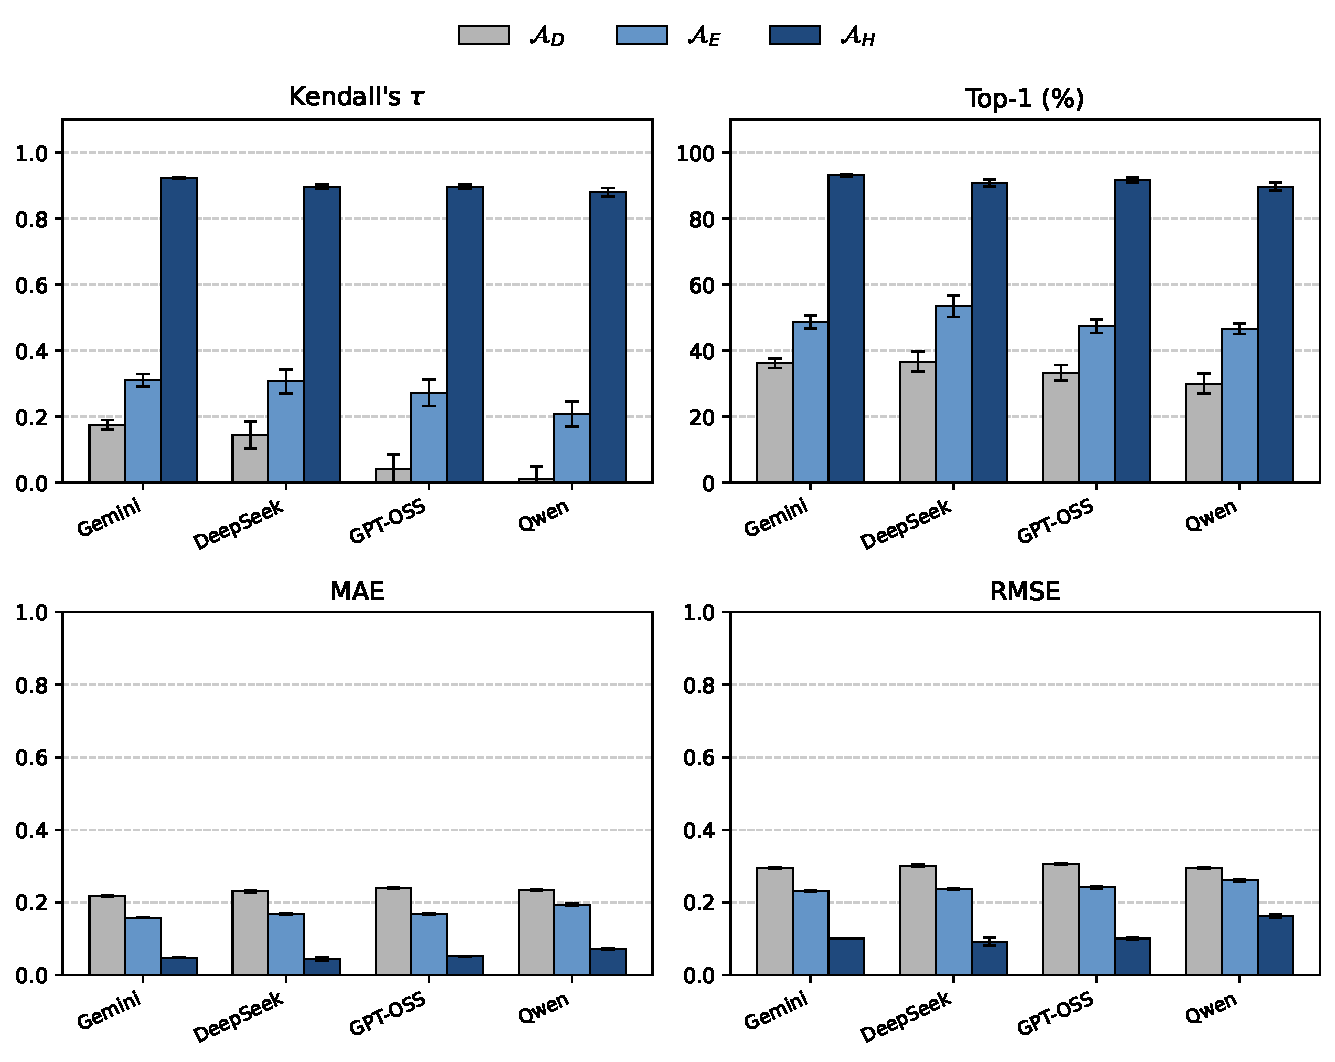
\includegraphics[width=0.68\textwidth]{OverallPerformanceByModel.pdf}
\caption{Overall accuracy by model and architecture.}
\label{fig:grouped_bars}
\end{figure}

Mean score error exceeds 0.2 for $\mathcal{A}_{\text{D}}$ in every model and lies between 0.045 and 0.072 for $\mathcal{A}_{\text{H}}$ (Figure~\ref{fig:grouped_bars}). Direct LLM scoring also spreads its scores too widely: its within-scenario score range is 1.25--2.00 times the reference's across models. We compare each architecture's spread with the reference's for the strongest and weakest model in Table~\ref{tab:dispersion}.

\begin{table}[htbp]
\caption{Within-scenario score dispersion for the strongest and weakest model.}
\label{tab:dispersion}
\centering
\begin{threeparttable}
  \centering
  \footnotesize
  \begin{tabular}{llccc}
    \toprule
    & & MAVT aggregate & \multicolumn{2}{c}{HVAC criterion range} \\
    \cmidrule(lr){4-5}
    Model & Architecture & range & Energy Cost & Comfort \\
    \midrule
    Reference & --- & 0.145 & 0.082 & 0.417 \\
    \midrule
    Gemini 3.5 Flash (best) & $\mathcal{A}_{\text{D}}$ & 0.233 $\pm$ 0.002 & 0.518 $\pm$ 0.008 & 0.547 $\pm$ 0.007 \\
     & $\mathcal{A}_{\text{E}}$ & 0.202 $\pm$ 0.004 & 0.489 $\pm$ 0.006 & 0.513 $\pm$ 0.004 \\
     & $\mathcal{A}_{\text{H}}$ & 0.141 $\pm$ 0.000 & 0.088 $\pm$ 0.001 & 0.417 $\pm$ 0.000 \\
    \addlinespace
    Qwen3.5 9B (worst) & $\mathcal{A}_{\text{D}}$ & 0.181 $\pm$ 0.011 & 0.240 $\pm$ 0.026 & 0.234 $\pm$ 0.013 \\
     & $\mathcal{A}_{\text{E}}$ & 0.175 $\pm$ 0.008 & 0.204 $\pm$ 0.012 & 0.260 $\pm$ 0.008 \\
     & $\mathcal{A}_{\text{H}}$ & 0.143 $\pm$ 0.001 & 0.096 $\pm$ 0.002 & 0.417 $\pm$ 0.001 \\
    \bottomrule
  \end{tabular}
  \begin{tablenotes}
    \item Mean over the 195 Test scenarios of the within-scenario range (maximum minus minimum across the three alternatives), on the 0--1 score scale. Architecture entries are the five-run mean $\pm$ standard deviation across runs; the reference is deterministic and has no run spread. We exclude scenarios with a failed score. We define best and worst model by mean Kendall's $\tau$ across all three architectures. A range wider than the reference's means the architecture separates the alternatives more than the physics warrants.
  \end{tablenotes}
\end{threeparttable}
\end{table}
\FloatBarrier

We break MAE down by criterion and model in Figure~\ref{fig:mae_criterion} (numerical values in Table S2.15). $\mathcal{A}_{\text{H}}$ has near-zero error on Comfort and Practicality for all four models. For all three architectures, error concentrates on Energy Cost and Environmental Impact, and on these two criteria $\mathcal{A}_{\text{H}}$'s weakest model outperforms the best models of $\mathcal{A}_{\text{D}}$ and $\mathcal{A}_{\text{E}}$. Which model does best on them depends on the decision type. Under $\mathcal{A}_{\text{H}}$, Gemini has the lowest error on HVAC (0.045 Energy Cost, 0.044 Environmental Impact) and Qwen the highest overall (0.112 and 0.150). Most of Qwen's error comes from Appliance, where its $\mathcal{A}_{\text{H}}$ Environmental Impact MAE of 0.294 still beats all four $\mathcal{A}_{\text{D}}$ models on the same criterion and decision type. Under $\mathcal{A}_{\text{D}}$, the models differ little (Energy Cost 0.241 to 0.258, Environmental Impact 0.248 to 0.292), and GPT-OSS and Qwen return the same score for Energy Cost and Environmental Impact on almost every Appliance alternative, the decision type on which the reference separates the two criteria most often (per-model shares in Table S2.14).

\begin{figure}[htbp]
	\centering
	\plotCriterionMAEByModel
	\caption{MAE by criterion, model and architecture.}
\label{fig:mae_criterion}
\end{figure}

\FloatBarrier
The results above cover only the scenarios that completed; we give the failure counts for each architecture and model in Table~\ref{tab:failure_arch_model}. Weighting each architecture's Kendall's $\tau$ by its success rate moves eleven of the twelve architecture--model cells by at most 0.004, consistent with their low failure counts. The exception is GPT-OSS under $\mathcal{A}_{\text{H}}$: its 88.0\% success rate lowers its success-weighted $\tau$ from 0.897 to 0.790 and its Top-1 from 91.7\% to 84.7\%. The $\mathcal{A}_{\text{H}} > \mathcal{A}_{\text{E}} > \mathcal{A}_{\text{D}}$ ordering still holds for all four models on the success-weighted metric; the narrowest margin is GPT-OSS's, at 0.790 against 0.272 for $\mathcal{A}_{\text{E}}$. A per-run imputed protocol gives the same ordering and the same single large movement (Table S2.13).

\begin{table}[htbp]
\caption{Failed scenario-runs by architecture and model, over five runs.}
\label{tab:failure_arch_model}
\centering
\begin{threeparttable}
\small\centering
\begin{tabular}{lccccc}
\toprule
Architecture & Gemini & DeepSeek & GPT-OSS & Qwen & Total \\
\midrule
$\mathcal{A}_{\text{D}}$ & 0 & 7 & 0 & 2 & 9 \\
$\mathcal{A}_{\text{E}}$ & 10 & 0 & 0 & 0 & 10 \\
$\mathcal{A}_{\text{H}}$ & 0 & 1 & 117 & 2 & 120 \\
\bottomrule
\end{tabular}
\end{threeparttable}
\end{table}

GPT-OSS accounts for 117 of the 120 $\mathcal{A}_{\text{H}}$ failures, most of them on HVAC scenarios (Table S1.5), while DeepSeek, Gemini and Qwen recorded at most two each across five runs. $\mathcal{A}_{\text{D}}$ and $\mathcal{A}_{\text{E}}$ fail mostly on unparseable output, whereas every $\mathcal{A}_{\text{H}}$ failure is an extracted parameter outside its physical validation bounds. GPT-OSS's failures also fall on different scenarios from run to run, and only one scenario failed in all five runs. When we recover each failed scenario from a run in which it succeeded, the reported figures do not change ($\tau$ 0.897, Top-1 91.7\%).

\FloatBarrier
\subsection{Where Does the Advantage Come From?}
\label{sec:res-extraction}
LLM-parameterized reference scoring hands the arithmetic to the calculator and keeps one step for the model: reading the withheld engineering parameters out of the scenario description. For each withheld numeric parameter, we report two quantities in Table~\ref{tab:extraction_accuracy}: the mean absolute extraction error, in the parameter's own units, and the probability that an error changes the alternative we would recommend. To compute the second, we re-ran the calculator on every scenario in which a model extracted a given parameter wrongly, substituting the extracted value for that parameter alone and holding every other parameter at its true value, and recorded how often the top-ranked alternative changed. This statistic measures the cost of an error rather than how often errors occur, so a parameter the models rarely get right can still score zero if the ranking does not depend on it.

\begin{table}[htbp]
\caption{Extraction error and its effect on the top-ranked alternative, by numeric hidden parameter.}
\label{tab:extraction_accuracy}
\centering
\begin{threeparttable}
\centering
\footnotesize
\renewcommand{\arraystretch}{1.15}
\setlength{\tabcolsep}{4pt}
\begin{tabular}{llcccccccc}
\toprule
 & & \multicolumn{4}{c}{MAE} & \multicolumn{4}{c}{$P(\text{Top-1 change} \mid \text{error})$} \\
\cmidrule(lr){3-6}\cmidrule(lr){7-10}
Type & Parameter & GPT-OSS & Qwen & DeepSeek & Gemini & GPT-OSS & Qwen & DeepSeek & Gemini \\
\midrule
HVAC & R-value & 3.594 & 3.699 & 2.312 & 1.766 & 0.015 & 0.086 & 0.015 & 0.000 \\
HVAC & SEER & 2.135 & 1.585 & 1.602 & 1.313 & 0.049 & 0.033 & 0.032 & 0.075 \\
HVAC & HVAC age (yr) & 8.5 & 6.1 & 8.5 & 7.6 & 0.000 & 0.000 & 0.000 & 0.000 \\
Appliance & kWh/cycle & 0.425 & 0.975 & 0.341 & 0.541 & 0.016 & 0.066 & 0.016 & 0.031 \\
Shower & GPM & 0.256 & 0.271 & 0.368 & 0.367 & \textbf{0.174} & \textbf{0.167} & \textbf{0.185} & \textbf{0.233} \\
Shower & Tank size (gal) & 8.1 & 8.9 & 6.9 & 6.7 & 0.000 & 0.026 & 0.025 & 0.000 \\
Shower & Heater setpoint (\textdegree{}F) & 4.7 & 4.6 & 8.3 & 4.6 & 0.042 & 0.050 & 0.042 & 0.050 \\
\bottomrule
\end{tabular}
\setlength{\tabcolsep}{6pt}
\renewcommand{\arraystretch}{1.0}
\end{threeparttable}
\end{table}

Extraction error varies widely by parameter. The models misestimate HVAC equipment age by 6.1--8.5 years on average and shower tank size by 6.7--8.9 gallons, both large fractions of their plausible ranges. The three categorical hidden parameters (appliance type, baseline run time and HVAC occupancy context) are either right or wrong, so we report match accuracy for them. All four models recover appliance baseline run time exactly, and three of the four recover appliance type exactly, with Gemini missing 4 of 65 cases (93.8\%). HVAC occupancy context has the lowest match accuracy, at 75.4\% for GPT-OSS, 78.6\% for Qwen, 80.0\% for Gemini and 81.4\% for DeepSeek, because the model must infer it from the phrasing of the question instead of reading it from a field. These errors rarely reach the decision. For most parameters, the probability that an extraction error changes the top-ranked alternative is below 0.09, and for HVAC equipment age it is zero for every model. Shower GPM is the consistent exception, with the highest probability for every model (0.167--0.233), roughly two to four and a half times that of the next-largest parameter; Section~\ref{sec:interpretation} explains why.

Two features of the design favor this result. With only three alternatives, correlated errors cancel more often than they would in a larger choice set, and per-scenario $\tau$ is coarse (Section~\ref{sec:eval-metrics}). The per-model $\tau$ of 0.880--0.923 therefore likely overstates $\mathcal{A}_{\text{H}}$'s ranking accuracy for larger choice sets.

\FloatBarrier
\subsection{Where Does It Break Down?}
\label{sec:res-bytype}
Performance differs by decision type, and LLM-parameterized reference scoring is weakest on Shower, the decision type that contains the GPM parameter. We give ranking accuracy by decision type in Table~\ref{tab:item7}, averaged over five runs, for the best and worst model in each cell (G for Gemini, D for DeepSeek, O for GPT-OSS, Q for Qwen), and the full per-model breakdown in Figure S2.4. $\mathcal{A}_{\text{H}}$ outperforms the other two architectures on all three decision types for every model. Even on Shower, where GPM errors change the recommendation most often (Section~\ref{sec:res-extraction}), it stays ahead of the other architectures for every model, though by only 0.055 in $\tau$ over $\mathcal{A}_{\text{E}}$ for Gemini.

\begin{table}[htbp]
\caption{Ranking accuracy by decision type, best and worst model.}
\label{tab:item7}
\centering
\begin{threeparttable}
\centering
\footnotesize
\renewcommand{\arraystretch}{1.15}
\setlength{\tabcolsep}{4pt}
\begin{tabular}{lcccccc}
\toprule
 & \multicolumn{2}{c}{$\mathcal{A}_{\text{D}}$} & \multicolumn{2}{c}{$\mathcal{A}_{\text{E}}$} & \multicolumn{2}{c}{$\mathcal{A}_{\text{H}}$} \\
\cmidrule(lr){2-3}\cmidrule(lr){4-5}\cmidrule(lr){6-7}
Decision Type & $\tau$ & Top-1 (\%) & $\tau$ & Top-1 (\%) & $\tau$ & Top-1 (\%) \\
\midrule
HVAC & & & & & & \\
\quad Best & 0.135 (O) & 39.7 (O) & 0.265 (O) & 46.9 (O) & \textbf{0.977 (G)} & \textbf{96.6 (G)} \\
\quad Worst & $-0.102$ (D) & 19.8 (D) & $-0.116$ (G) & 15.3 (G) & \textbf{0.881 (Q)} & \textbf{87.4 (Q)} \\
Appliance & & & & & & \\
\quad Best & 0.029 (D) & 31.7 (D) & 0.417 (D) & 70.2 (D) & \textbf{0.975 (D)} & \textbf{98.5 (D)} \\
\quad Worst & $-0.147$ (O) & 26.8 (O) & $-0.048$ (O) & 30.5 (O) & \textbf{0.906 (Q)} & \textbf{92.9 (Q)} \\
Shower & & & & & & \\
\quad Best & 0.633 (G) & 61.0 (G) & 0.767 (G) & 79.3 (G) & \textbf{0.851 (Q)} & \textbf{89.0 (Q)} \\
\quad Worst & 0.069 (Q) & 34.3 (Q) & 0.240 (Q) & 47.0 (Q) & \textbf{0.787 (D, tied with O)} & \textbf{81.0 (D)} \\
\bottomrule
\end{tabular}
\begin{tablenotes}
\footnotesize
\item We choose the best and worst model in each cell by Kendall's $\tau$; Top-1 is that model's value.
\end{tablenotes}
\setlength{\tabcolsep}{6pt}
\renewcommand{\arraystretch}{1.0}
\end{threeparttable}
\end{table}

$\mathcal{A}_{\text{E}}$ varies widely across models on HVAC ($\tau$ from $-0.116$ to $0.265$) and performs best on Shower for every model ($\tau$ from $0.240$ to $0.767$). The gap between $\mathcal{A}_{\text{H}}$ and $\mathcal{A}_{\text{E}}$ is narrowest on Shower, whose three alternatives differ only in duration, for every model, and widest on HVAC for every model except GPT-OSS, whose widest gap is on Appliance. $\mathcal{A}_{\text{D}}$ is near chance or below on HVAC and Appliance for every model. On Shower, the two strongest models reach moderate agreement with the reference (Gemini $\tau = 0.633$, DeepSeek $\tau = 0.558$), while the two weakest stay near chance (GPT-OSS $\tau = 0.133$, Qwen $\tau = 0.069$).

\FloatBarrier
\subsection{Sensitivity and Robustness}
\label{sec:res-sensitivity}
Differences of this size could come from choices we made rather than from the architectures themselves. We varied five of those choices (Section~\ref{sec:ablation-design}), and none of them changes the architecture ordering within a model except in one weight-vector cell. Full statistics for every check are in Supplementary Material S2.

Reversing the alternative order changed $\mathcal{A}_{\text{D}}$'s Top-1 accuracy by fewer than 9 of 195 scenarios, net, for every model, and no shift reaches significance (the closest, DeepSeek, has a median McNemar $p = 0.477$). For $\mathcal{A}_{\text{H}}$, reversal moved the extracted parameters for two of the four models (Qwen and Gemini), both at the test's floor of $1/1287$, but changed no model's top-ranked alternative, and the two conditions differ by less than $0.004$ in Kendall's $\tau$. The calculator's error cancellation absorbs the perturbation before it reaches the ranking.

Prompt wording does not change the architecture ordering within any model: every $\mathcal{A}_{\text{E}}$ variant stays above every $\mathcal{A}_{\text{D}}$ variant on Kendall's $\tau$. Under $\mathcal{A}_{\text{E}}$, no perturbation improved on the original prompt. Under $\mathcal{A}_{\text{D}}$, the two significant comparisons, both for Qwen and both favoring the perturbation, fall between $\tau = -0.052$ and $\tau = 0.092$, so they separate one near-random ranking from another. The choice of model can still outweigh the architecture: under the rescaled-response variant, $\mathcal{A}_{\text{E}}$ with Qwen ($\tau = 0.102$) falls below $\mathcal{A}_{\text{D}}$ with DeepSeek ($\tau = 0.167$).

Retrieval configuration matters for DeepSeek and Gemini only; for GPT-OSS and Qwen the seven configurations are indistinguishable after Holm correction. Removing the reference scores from the exemplars lowers $\tau$ for every model, while removing the hidden engineering parameters moves it in both directions and by less, except for Qwen (Figure~\ref{fig:rag_ablation}). Score accuracy responds before ranking does: removing the scores or drawing random exemplars raises MAE by about half for DeepSeek, GPT-OSS and Qwen and doubles it for Gemini. Retrieving one exemplar instead of three costs Gemini, GPT-OSS and Qwen nothing we can measure, but costs DeepSeek $0.32$ in $\tau$.

\FloatBarrier
\begin{figure}[htbp]
	\centering
	\plotRagAblation
	\caption{Kendall's $\tau$ by retrieval configuration (90 RAG scenarios, leave-one-out).}
\label{fig:rag_ablation}
\end{figure}

The ordering $\mathcal{A}_{\text{H}} > \mathcal{A}_{\text{E}} > \mathcal{A}_{\text{D}}$ holds at every value of the curvature parameter $\alpha$ for every model, and $\mathcal{A}_{\text{H}}$'s $\tau$ changes by less than 0.02 across the sweep, even though the sweep moves the reference away from $\mathcal{A}_{\text{H}}$'s fixed scores.

Under the alternative weight vectors, $\mathcal{A}_{\text{H}}$ stays ahead of $\mathcal{A}_{\text{E}}$ in all 20 model--weight-vector cells, by at least $0.304$ in Kendall's $\tau$. $\mathcal{A}_{\text{E}}$'s lead over $\mathcal{A}_{\text{D}}$ holds under the equal and entropy vectors for all four models, shrinks under the MEREC vectors, and reverses in one cell: under the MEREC HVAC vector, Gemini's $\mathcal{A}_{\text{D}}$ overtakes its $\mathcal{A}_{\text{E}}$ ($0.676$ vs.\ $0.600$). The MEREC vectors load onto Comfort, the one criterion that $\mathcal{A}_{\text{D}}$ estimates about as well as $\mathcal{A}_{\text{E}}$.

\FloatBarrier
\subsection{Efficiency and Cost}
\label{sec:res-efficiency}
A practitioner also weighs cost, so we report API cost and token use per run for every architecture and model in Table~\ref{tab:item8}, averaged over five runs (prices and their date in Supplementary Material S1). Because $\mathcal{A}_{\text{H}}$ makes one API call per scenario against three for the other two architectures, it is the cheapest architecture for every model: $\mathcal{A}_{\text{D}}$ costs 2.9--7.9 times as much as $\mathcal{A}_{\text{H}}$ on the same model, and $\mathcal{A}_{\text{E}}$ 3.3--3.8 times as much. Per-run cost ranges from \$0.006 (GPT-OSS with $\mathcal{A}_{\text{H}}$) to \$1.024 (Gemini with $\mathcal{A}_{\text{E}}$).

\begin{table}[htbp]
\caption{Cost per run (USD) and total tokens per run (thousands, input+output).}
\label{tab:item8}
\centering
\begin{threeparttable}
\centering
\small
\renewcommand{\arraystretch}{1.15}
\setlength{\tabcolsep}{4pt}
\begin{tabular}{l cc cc cc cc}
\toprule
 & \multicolumn{2}{c}{Gemini} & \multicolumn{2}{c}{DeepSeek} & \multicolumn{2}{c}{GPT-OSS} & \multicolumn{2}{c}{Qwen} \\
\cmidrule(lr){2-3}\cmidrule(lr){4-5}\cmidrule(lr){6-7}\cmidrule(lr){8-9}
Architecture & Cost & Tokens & Cost & Tokens & Cost & Tokens & Cost & Tokens \\
\midrule
$\mathcal{A}_{\text{D}}$ & \$0.802 & 414.2k & \$0.087 & 667.7k & \$0.023 & 493.1k & \$0.043 & 423.6k \\
$\mathcal{A}_{\text{E}}$ & \$1.024 & 428.7k & \$0.036 & 384.4k & \$0.023 & 482.5k & \$0.042 & 407.6k \\
$\mathcal{A}_{\text{H}}$ & \$0.280 & 113.3k & \$0.011 & 110.2k & \$0.006 & 122.7k & \$0.012 & 112.4k \\
\bottomrule
\end{tabular}
\setlength{\tabcolsep}{6pt}
\renewcommand{\arraystretch}{1.0}
\end{threeparttable}
\end{table}

\FloatBarrier
\section{Discussion}
\label{sec:discussion}

When interpreting these results, we keep three points in mind. First, LLM-parameterized reference scoring's advantage comes from the structure of the decision rather than from the accuracy of its extraction. Second, the architecture that ranks best is also the cheapest to run. Third, a calculator driven by fixed constants, with no LLM at all, already matches or beats LLM-parameterized reference scoring for two of the four models on two of the three decision types (HVAC and Shower), which limits how much the language model can contribute.

\FloatBarrier
\subsection{Interpretation of Results}
\label{sec:interpretation}
$\mathcal{A}_{\text{H}}$ was the strongest architecture overall and the only one whose within-scenario score spread matched the reference calculator's (0.140--0.150 across models, against 0.145). The wider spread of the other two architectures is consistent with the scoring biases that \citet{li2026scoringbias} found in LLM-as-judge pipelines; $\mathcal{A}_{\text{H}}$ avoids those biases because its LLM does no scoring. Converting each architecture's criterion MAE back through the reference ranges of Table~\ref{table:reference_ranges} expresses the error in physical units. Across the four models, $\mathcal{A}_{\text{H}}$ misses by \$0.09--\$0.16 per scenario on Energy Cost, by 0.6--1.3 lbs CO\textsubscript{2} on HVAC and Appliance, and by 2--3 gallons of water on Shower; $\mathcal{A}_{\text{E}}$ misses by \$0.27--\$0.34, 1.7--2.4 lbs and 3--7 gallons. Model capability also matters least under $\mathcal{A}_{\text{H}}$ (Section~\ref{sec:res-ranking}).

Extraction error rarely reaches the ranking, and the reason is the structure of the decision rather than the accuracy of the extraction. If $\mathcal{A}_{\text{H}}$ extracts a house's insulation as R-14 when the true value is R-16, the underestimate raises the projected heating loss, and with it the cost and emissions estimate, for all three setpoint alternatives under comparison; the alternative that was cheapest at the true R-16 is still cheapest at the estimated R-14, because the error moves every alternative in the same direction rather than reordering them. The cancellation fails only when another alternative is close to winning on Comfort or Practicality.

The cancellation depends on the alternatives sharing the same uncertain state, such as a house's insulation, which then scales their cost and emissions alike. It weakens for a parameter that scales the outcome directly and that the model must recover from a coarse proxy. Shower GPM is that parameter (Section~\ref{sec:res-extraction}): cost and water use are both proportional to GPM times duration, so a GPM error rescales the gaps between the three durations on those two criteria without reordering them, while the Comfort gaps, which do not depend on GPM, stay fixed; when the reference winner leads narrowly, the rescaled gaps are enough to change it. We would expect a multiplier of the same kind in another domain, such as a per-unit rate in a financial decision, to break it the same way.

The same two models fail across tests that have nothing to do with each other. GPT-OSS carries 117 of the 120 $\mathcal{A}_{\text{H}}$ extraction failures, every one of them a parameter outside the physical bounds, so its weakness there is a failure to stay in range rather than a failure to estimate close to the true value. Under $\mathcal{A}_{\text{D}}$, GPT-OSS and Qwen return identical Energy Cost and Environmental Impact scores for 93.7\% and 95.6\% of Appliance alternatives against the reference's own 8.0\% (Table S2.14): neither separates the two criteria, although we instruct them to. Where the quantities are collinear that collapse costs little, but it shows that the models do not reason about the two scores separately. Qwen ranks last under every architecture, and neither architecture that asks it to score works well for it. Under $\mathcal{A}_{\text{H}}$, the result depends far less on model strength than under $\mathcal{A}_{\text{D}}$ and $\mathcal{A}_{\text{E}}$. Gemini shows the converse: it varies least between runs and leads on $\mathcal{A}_{\text{H}}$, yet it is the only model with any $\mathcal{A}_{\text{E}}$ failures and the only one whose $\mathcal{A}_{\text{D}}$ overtakes $\mathcal{A}_{\text{E}}$ under any weight vector (Section~\ref{sec:res-sensitivity}), so stability across runs does not imply stability across architectures.

The architecture that ranks best is also the cheapest to run, by roughly three to eight times on the same model, because it makes one API call per scenario against three for the other two (Section~\ref{sec:res-efficiency}). For a practitioner, accuracy and cost point the same way. Where a deterministic calculator exists for the decision type, asking the model to score the alternatives directly is generally the worst option on both counts: it is the least accurate architecture for every model and costs more than LLM-parameterized reference scoring, though for Gemini it costs less than example-guided LLM scoring and for GPT-OSS the same.

Example-guided LLM scoring corrects the level of the model's scores more than its ability to separate the alternatives. A few scored examples show the model what range the reference scale covers, but not how to compute a new scenario's own numbers, so the model recalibrates its baseline while gaining only part of the discrimination the reference has. Every model improves: under $\mathcal{A}_{\text{E}}$, $\tau$ ranges from 0.208 to 0.310 across the four models, against 0.010 to 0.176 under $\mathcal{A}_{\text{D}}$. Even at its best, $\mathcal{A}_{\text{E}}$ stays far below $\mathcal{A}_{\text{H}}$ (Section~\ref{sec:res-ranking}), so exemplars narrow the numeracy gap of direct LLM scoring without closing it.

In the RAG ablation, the scores in the exemplars matter and the additional household information matters little (Section~\ref{sec:res-sensitivity}, Figure~\ref{fig:rag_ablation}). Exemplars also narrow the spread of the scores: DeepSeek's within-scenario range falls from 0.289 under $\mathcal{A}_{\text{D}}$ to 0.162 under $\mathcal{A}_{\text{E}}$, and Qwen's from 0.181 to 0.175. Retrieving similar examples, rather than any examples, provides most of what retrieval contributes. Qwen is the exception: its Kendall's $\tau$ under random exemplars (0.276) exceeds its $\tau$ under the similarity-ranked $k=3$ exemplars (0.154; Table S2.5). Qwen is the smallest model we tested and may use the exemplar scores as a formatting template rather than reasoning about them, in which case its higher $\tau$ under random exemplars is no evidence about retrieval quality.

$\mathcal{A}_{\text{D}}$ fails in a way the LLM-as-judge literature does not predict. It sits near chance on HVAC and Appliance for all four models and separates on Shower only for the two strongest (Gemini $\tau = 0.633$, DeepSeek $0.558$, against GPT-OSS $0.133$ and Qwen $0.069$; Section~\ref{sec:res-bytype}), consistent with Shower's single dominant duration trade-off being easier for a capable model to reason about directly than HVAC's or Appliance's multi-parameter interactions (elaborated in Section~\ref{sec:comparison}).

The entropy weights come close to the assumed 35/30/20/15 weights; MEREC-derived weights instead emphasize the criteria that distinguish the alternatives at hand. Under those vectors, $\mathcal{A}_{\text{E}}$ loses most of its margin over $\mathcal{A}_{\text{D}}$ (Section~\ref{sec:res-sensitivity}; full matrix in Tables S2.2 and S2.3). Every entropy vector puts a combined 0.64--0.66 on Energy Cost and Environmental Impact against the design's 0.65, and that shared emphasis keeps the ordering intact. $\mathcal{A}_{\text{E}}$'s advantage over $\mathcal{A}_{\text{D}}$ therefore depends on emphasizing cost and emissions, the criteria that direct LLM scoring estimates poorly. Both criteria require converting a physical quantity into a dollar or emissions figure through several multiplicative steps, an implicit calculation that direct and exemplar-anchored scoring alike must perform within one response, with at most a low-effort reasoning trace, unlike the more categorical judgments that Comfort and Practicality require.

The fixed-default baseline performs well only where its defaults happen to suit the decision (Section~\ref{sec:res-baselines}). It collapses on Appliance ($\tau = 0.097$) because Practicality alone recovers the reference winner in 90.8\% of Appliance scenarios, and a fixed 7\,p.m.\ run time cannot track a household's actual schedule, which is what Practicality measures. $\mathcal{A}_{\text{H}}$ clears the fixed default overall and on Appliance for every model. On HVAC ($\tau = 0.933$ for the fixed default) and Shower ($\tau = 0.800$), it clears the default for only two of the four models each: Gemini and GPT-OSS on HVAC, Gemini and Qwen on Shower. On HVAC, an R-15, SEER-13 default sits near the typical values of the Pennsylvania housing stock these scenarios draw on. $\mathcal{A}_{\text{E}}$ falls below the fixed default on overall Kendall's $\tau$ and on HVAC and Shower for all four models, and beats it on Appliance for every model except GPT-OSS. These results describe how closely the defaults match this dataset's housing stock; we would not expect a default tuned to a different climate zone or building-code era to clear the same bar.

\FloatBarrier
\subsection{What These Results Confirm and Qualify}
\label{sec:comparison}

Our direct-LLM-scoring results qualify prior claims that internal consistency implies correct output: \citet{svoboda2024} showed GPT-4 can construct an AHP model within consistency-ratio thresholds and \citet{icaart26} found that the COMET decomposition makes LLM rankings more stable than direct LLM ranking, yet in our case $\mathcal{A}_{\text{D}}$, across multiple runs, had low-variance scores while still being far from correct (Section~\ref{sec:res-ranking}). This miscalibration extends the scoring biases that \citet{wang2024fairescalers} and \citet{li2026scoringbias} documented from judge contexts to multi-criteria decision scoring. $\mathcal{A}_{\text{D}}$'s within-scenario range runs 1.25--2.00 times the reference range (Section~\ref{sec:res-ranking}). A model asked to score alternatives on a bounded scale can spread its scores as easily as it can compress them, so calibrating against scores that are ``too average'' can backfire.

With $\mathcal{A}_{\text{E}}$, we extend case-based reasoning \cite{aamodtplaza1994,minorkaucher2024} to MCDA scoring, but its gain over $\mathcal{A}_{\text{D}}$ levels off because exemplar scores anchor the output scale without correcting the model's scenario-specific arithmetic (Section~\ref{sec:res-ranking}). $\mathcal{A}_{\text{H}}$ avoids the arithmetic weakness that \citet{imani2023mathprompter} documented by using a single extraction call and an existing calculator, instead of trying to improve the model's arithmetic through chain-of-thought prompting \cite{wei2022cot} or self-verification.

\citet{vonnitzsch1993} showed that importance weights elicited without reference to the attribute ranges on offer differ systematically from swing weights elicited with them; the 35/30/20/15 vector used here is of the first kind (Section~\ref{sec:res-sensitivity}; the criterion swings realized in the scenario set are in Table S2.1). \citet{vahidnia2025walmas} take the opposite approach and ask an LLM to assign the weights themselves. From these two studies we can draw a decomposition this paper leaves untested: an LLM could supply the weights, the withheld parameters, or the scores, and we vary only the last two.

\citet{goodell2025} found the same three-way ordering in clinical calculation (Section~\ref{sec:lit-numeracy}). Two groups working independently, in different domains, have now found the same ordering; \citet{goodell2025} read the convergence of several research groups on clinical calculation as evidence both that current LLMs calculate unreliably and that tool augmentation is a promising remedy, and our results add a second domain to that evidence. Their error taxonomy makes a more specific prediction: tool augmentation removes criteria, formula and calculation errors, while interpretation errors remain. We find the same pattern independently. The lowest categorical extraction accuracy in this study is HVAC occupancy context, at 75.4\% for GPT-OSS, 78.6\% for Qwen, 80.0\% for Gemini and 81.4\% for DeepSeek (Section~\ref{sec:res-extraction}). Occupancy context is the one parameter a model must read from the phrasing of the question rather than look up in a scenario field, which is the error class their taxonomy predicts a calculator cannot remove. \citet{goodell2025} did not test whether an error would have changed the patient's management, and they name that test as future work. We run it for a ranking: the probability that an extraction error changes the top-ranked alternative (Table~\ref{tab:extraction_accuracy}).
\FloatBarrier
\subsection{Limitations of the Study}
\label{sec:limitations}

We grade $\mathcal{A}_{\text{H}}$ against the same calculators it uses. $\mathcal{A}_{\text{H}}$ uses the reference model's calculator but does not receive several of its inputs, which it must estimate from homeowner-accessible text; we took the physical validation bounds (R-value, SEER and GPM ranges) from ASHRAE and ENERGY STAR literature rather than from pilot LLM outputs. A misspecified formula would inflate $\mathcal{A}_{\text{H}}$'s accuracy and could lower the other two architectures'. An independent audit with a separately built calculator would resolve this (Section~\ref{sec:futurework}). $\mathcal{A}_{\text{H}}$ is also limited to what the calculator models: if a criterion the calculator cannot represent becomes important, such as indoor humidity for an HVAC decision, which ASHRAE~55's temperature-only comfort model does not include, $\mathcal{A}_{\text{H}}$ falls back on the same weaknesses as the other two architectures. Several calculator relationships are unpublished, or we cannot check them against the scenario data: mains water temperature interpolated linearly from outdoor temperature \cite{burch2007}, monthly appliance cycle rates, a fixed shower tank-availability factor of 0.8, and a run-time-fraction approximation for HVAC occupancy. These affect all architectures equally, but the absolute MAE and RMSE values combine LLM extraction error with calculator imputation error.

We calibrated each criterion's 0--1 scoring curve against published standards and population-level data rather than eliciting it from any household, so the reference ranking describes a normative, reasonable household rather than any particular household's trade-offs. A homeowner who weighs Comfort above its 20\% weight, tolerates a colder shower than ASHRAE~55 predicts, or works a shift that rules out a daytime wash would need an adjusted calculator; we take up what that means for distribution in Section~\ref{sec:conclusion}. The nominal weights act as fixed importance weights rather than range-sensitive swing weights, and we assume a single decision-maker holds them. Generalizing to nearby alternatives also assumes monotonicity, which holds for cost and energy but not always for Comfort.

We generated the scenario dataset by crossing categorical parameters with representative numeric draws, which covers the parameter space but does not reproduce the joint distributions found in real housing: older houses tend to have both worse insulation and lower SEER ratings, and the synthetic dataset decouples the two. Accuracy in real-world use may therefore be lower.

Results are specific to Pennsylvania's grid and utility rate structure: the PJM marginal emissions factors and Pennsylvania time-of-use rate tiers used throughout this study do not generalize to high-renewables grids, where lower and more variable emissions intensities would compress environmental score distributions, and absolute MAE values for the Environmental Impact and Energy Cost criteria would shift. One consequence matters for the criterion set: because the three alternatives of an HVAC or Shower scenario share one time of use, and Shower cost and water volume both scale with duration, the four-criterion specification collapses to an effective three on HVAC and Shower, with 0.65 of the weight resting on a single cost/emissions dimension (Section~\ref{sec:criteria-weighting}). We also assume electric resistance water heating in every Shower scenario.

\FloatBarrier
\subsection{Future Work}
\label{sec:futurework}
The most immediate follow-up is an external review of $\mathcal{A}_{\text{H}}$'s extraction schema and validation bounds. A household-decision expert could score a sample of scenarios without seeing the calculator's output, which would test the reference ranking against human judgment.

Cross-grid replication under different emissions--cost correlation structures (e.g., ERCOT or a high-nuclear European grid) would address the PJM specificity noted in Section~\ref{sec:limitations}. A domain-transfer test would apply $\mathcal{A}_{\text{H}}$ to a mature calculator outside energy (e.g., actuarial life-expectancy or portfolio Sharpe-ratio estimation). A domain whose decision rules are less consistent than household physics would show where $\mathcal{A}_{\text{H}}$'s advantage degrades.

None of the three architectures produces a calibrated confidence estimate alongside its ranked recommendation, so a correct ranking and an inverted one reach the household in the same form. Attaching a confidence signal calibrated against the reference, and measuring whether households act on it, is a prerequisite for deployment. Longer-term extensions include multi-turn preference elicitation from multiple household members and a randomized controlled trial comparing LLM-MCDA recommendations against unaided decisions in deployed households.

\FloatBarrier
\section{Conclusion}
\label{sec:conclusion}
We benchmarked three strategies for integrating an LLM into an MCDA workflow against a deterministic MAVT reference across 195 household energy scenarios. The ordering $\mathcal{A}_{\text{H}} > \mathcal{A}_{\text{E}} > \mathcal{A}_{\text{D}}$ holds for every model tested. Our metrics measure fidelity to the specified reference model, not real-world decision accuracy.

A language model belongs in a pipeline that already has, or could have, a deterministic way to check its answer. The division of labor we set out in Section~\ref{sec:introduction} holds: the architecture that never asks the model to compute an outcome reproduces the reference, and the choice of model matters far less when the model only translates than when it scores.

An LLM is worth using as an interpreter once a deterministic calculator exists, and in some cases the calculator alone is already enough. Direct LLM scoring is the least accurate of the three architectures for every model and costs more than extracting parameters for a calculator, so where a calculator exists we see no reason to use it. A fixed default that substitutes one constant for each withheld parameter, with no per-scenario inference, outranks $\mathcal{A}_{\text{E}}$ on overall Kendall's $\tau$ for all four models at no LLM cost. The language model adds value only where a single average input would be badly wrong for the household in front of it.

We contribute an evaluation framework and an open reference implementation for MCDA with an LLM front end in residential energy: three deterministic MAVT calculators, a 285-scenario dataset split into 195 test and 90 retrieval cases, and a harness that reports Kendall's $\tau$, Top-1, MAE and RMSE per model and per decision type.

Because we calibrated the reference curves to a normative household rather than a particular one (Section~\ref{sec:limitations}), $\mathcal{A}_{\text{H}}$ as built suits only the households those curves already describe. Retrieving exemplars scored under a household's own revealed preferences, in the style of $\mathcal{A}_{\text{E}}$, is the more plausible route to a system a household could adopt unchanged, and from our retrieval results we can anticipate what such a system would and would not inherit. A more dynamic pipeline, in which the household works out its preferences with the model at each use, is the other route worth trying.

\clearpage

\paragraph*{Declaration of competing interest}
The authors declare that they have no known competing financial interests or personal relationships that could have appeared to influence the work reported in this paper.

\paragraph*{Funding}
This research did not receive any specific grant from funding agencies in the public, commercial, or not-for-profit sectors.

\paragraph*{CRediT authorship contribution statement}
\textbf{Ahaan Nigam:} Conceptualization, Methodology, Software, Validation, Formal analysis, Investigation, Data Curation, Writing --- Original Draft, Writing --- Review \& Editing, Visualization. \textbf{River Huang:} Validation, Conceptualization, Methodology, Supervision, Writing --- Review \& Editing.

\paragraph*{Software and data availability}
Name of software/dataset: LLM-MCDA-Paper (benchmark code, reference calculators, and scenario/RAG data). Access: \url{https://github.com/AN00927/LLM-MCDA-Paper}.
Developer and contact: Ahaan Nigam (\href{mailto:ishaannigam27@gmail.com}{ishaannigam27@gmail.com}). 
Year first available: 2026. 
Program language: Python.
Software required: Python 3.11 or newer and the packages listed in \texttt{requirements.txt}.
License: MIT. Cost: free.
The repository includes the per-run outputs of every model, so every table, figure and statistical test in this paper can be regenerated without an API key. Re-collecting the benchmark requires an API key for the model provider named in Supplementary Material S1 and incurs the costs in Table~\ref{tab:item8}.

\paragraph*{Declaration of generative AI and AI-assisted technologies in the manuscript preparation process}
During the preparation of this work, the authors used Anthropic's Claude (via the Claude Code CLI) and OpenAI's ChatGPT to assist with drafting, copy-editing manuscript text, graphical refinement, and conceptualizing/refining the graphical abstract illustrations. No text, data, numbers, or figures were accepted without manual verification. The authors reviewed and edited all content and take full responsibility for the content of the published article.

\paragraph*{Supplementary material}
Supplementary material associated with this article is available online. Part S1 (Extended Methods) contains the full parameter-comparison tables, the scenario-flow diagram, prompt texts, time-of-use rate structures, failure-mode analysis, and worked examples referenced from the main text; Part S2 (Extended Results and Robustness) contains the entropy and MEREC weight vectors, the per-decision-type results by model, and the sensitivity, RAG-ablation, variance, significance, imputation, aggregation, and numerical results tables and figures.

\bibliographystyle{elsarticle-num-names}
\bibliography{cas-refs}

\end{document}

